\documentclass[9pt,twocolumn,twoside,lineno]{pnas-new}
% Use the lineno option to display guide line numbers if required.
% Note that the use of elements such as single-column equations
% may affect the guide line number alignment. 

\templatetype{pnasresearcharticle} % Choose template 
% {pnasresearcharticle} = Template for a two-column research article
% {pnasmathematics} = Template for a one-column mathematics article
% {pnasinvited} = Template for a PNAS invited submission
\usepackage{amssymb,amsfonts,amsthm,bm}
\usepackage{adjustbox}
\usepackage[round,numbers,sort&compress]{natbib}
\usepackage{graphicx}
\usepackage{amssymb}
\usepackage{fixltx2e}
\usepackage{graphicx}
\usepackage{wrapfig, blindtext}
\usepackage{setspace} 

\begin{document}
\title{Cross-pore electrostatic repulsions are critical for stabilizing the GABA\textsubscript{A} receptor open state}
\title{The golden ratio in ion channel gating: Spontaneous pore opening in GABA\textsubscript{A} receptors}
\title{Spontaneous pore opening in GABA\textsubscript{A} receptors from electrostatics with pentagonal symmetry }
\title{Allostery from a charged pentagon: Spontaneous pore opening in warm GABA\textsubscript{A} receptors  }
\title{Allostery in GABA\textsubscript{A} receptors via noisy dipole and flexible charged pentagon  }
\title{Viewable allostery in warm GABA\textsubscript{A} receptors }
\title{Multibody interactions lead to conformational selection of an open state in warm GABA\textsubscript{A} receptors }
\author[a,1]{Sruthi Murlidaran}
\author[a,b,2]{Reza Salari}
\author[a,b,3]{Grace Brannigan}

\affil[a]{Rutgers University, Center for Computational and Integrative Biology, Rutgers University, Camden, NJ, USA}
\affil[b]{Department of Physics, Rutgers University, Camden, NJ, USA}

\newcommand{\SFullABF}{S14}
\newcommand{\sfigAlignment}{S3}
\newcommand{\sfigDeltaPhiDist}{S2}
\newcommand{\SklowTrepTwo}{S6}
\newcommand{\SkMovie}{S1}
\newcommand{\sFigEnergy}{S1}
\newcommand{\sFigReplicas}{S5-S11}
\newcommand{\grace}[1]{\textcolor{blue}{#1}}
\newcommand{\GABAA}{GABA\textsubscript{A}R\xspace}
\newcommand{\avgr}{\bar{r}}
\newcommand{\varr}{\delta r^{2}}
\newcommand{\plgics}{pLGICs}
\newcommand{\plgic}{pLGIC~}
\newcommand{\nachr}{nAChR~}
%\newcommand{\fivering}{M2 24$^{\prime}$ ring~}
\newcommand{\fivering}{interfacial band~}
\newcommand{\fiveringnos}{interfacial band}
\newcommand{\triad}{pore oscillator~}
\newcommand{\triadns}{pore oscillator}
\newcommand{\extended}{elongated~}
%\newcommand{\rigid}{Rigid~}
%\newcommand{\compressed}{Rigid-Compressed~}
%\newcommand{\fuzzy}{Fuzzy~}
%\newcommand{\fuzcomp}{Fuzzy-Compressed~}
%\newcommand{\latch}{Latched-open~}
%\newcommand{\shut}{Latched-shut~}
%\newcommand{\stable}{stabilization~}
%\newcommand{\shift}{shift~}
%\newcommand{\stoch}{stochastic compression~}
%\newcommand{\recoil}{recoil~}
%\newcommand{\collapse}{collapse~}
\newcommand{\flip}{flip~}
\newcommand{\muthotmovie}{2}
%%


%\newcommand{\GABAA}{GABA\textsubscript{A}R\xspace}
%\newcommand{\avgr}{\bar{r}}
%\newcommand{\varr}{\delta r^{2}}
%\newcommand{\plgics}{pLGICs}
%\newcommand{\nachr}{nAChR}
\begin{abstract}$\gamma_2$
GABAA receptors are critical for proper transmission of inhibitory signals in the central nervous system, and are common targets of anesthetic and anxiolytic drugs. They are also members of the widely-studied pentameric ligand-gated ion channel family (pLGIC). Here we use a slightly increased temperature to, for the first time, observe a stable spontaneous opening event of a pLGIC in molecular simulation. We find the opening event reflects interactions in two rings of homologous charges in the receptor transmembrane domain, an "interfacial band" containing five basic residues at M2 24' in the M2-M3 loop, and the "pore oscillator" composed of two acidic residues and one basic residue at 20' on the two $\beta$ and one $\gamma$ M2 helices respectively. The pore oscillator is shown to drive fluctuations in pore radius, by switching between attractive and repulsive cross-pore electrostatic interactions, consistent with a classic Coulomb charge-dipole arrangement. A conformational change of the interfacial band from an asymmetric to a symmetric state locks the pore oscillator in a repulsive (open) configuration. The $\gamma_2$ K289M mutation is a rare mutation (rs121909672) that causes seizures with fever and also neutralizes the $\gamma_2$ residue in the interfacial band.  The electrostatic energy of an interfacial band with only four charges is shown to be more sensitive to random shape fluctuations, which increase with higher temperature. Our simulation results indicate these effects are also transmitted to the pore.  Temperature-enhanced fluctuations could thus cause rapid gating in these mutant receptors, consistent with flickering observed previously in single-channel recordings.%{GABA\textsubscript{A} receptors (\GABAA) are critical for proper transmission of inhibitory signals in the central nervous system, and are common targets of anesthetic and anxiolytic drugs.  
%They are members of the widely-studied pentameric ligand-gated ion channel family (pLGIC). Here we use a slightly increased temperature to, for the first time, observe a stable spontaneous opening event of a pLGIC in molecular simulation.  We find the opening event reflects interactions in two rings of homologous charges in the receptor transmembrane domain, an ``\fiveringnos'' containing five basic residues at M2 24$^{\prime}$ in the M2-M3 loop, and the ``\triadns`` composed of two acidic residues and one basic residue at 20$^{\prime}$ on the two $\beta$ and one $\gamma$ M2 helices respectively.  The \triadns~is shown to drive fluctuations in pore radius, by switching between attractive and repulsive cross-pore electrostatic interactions, consistent with a classic Coulomb charge-dipole arrangement.  A conformational change of the \fivering from an asymmetric to a symmetric state locks the \triad in a repulsive (open) configuration. %Dispersion of the charges in a symmetric \fivering increases with temperature without significantly affecting total electrostatic energy of the \fiveringnos as long as it is fully charged; 
%The electrostatic energy of an \fivering with only four charges is shown to be more sensitive to shape deformations, which increase with higher temperature. The $\gamma_{2}$K289M mutation is a rare mutation (rs121909672) that neutralizes the \fivering charge from the $\gamma_{2}$ subunit; it is associated with fever-induced seizures in humans and has been previously shown to cause flickering in single-channel recordings. Unbiased and Adaptive Biasing Force (ABF) molecular simulations of the K289M mutant indicate a shift toward closed states at higher temperatures; the shift is correlated to expected and observed effects on multibody interactions within the \fiveringnos.  %increased shape fluctuations of the partially charged \fiveringnos, as well as increased sensitivity of the pore conformation to \fiveringnos shape fluctuations.   
%For the stable open state, the interfacial band must have transitioned from a flexible elongated pentamer to a rigid regular one; this transition is energetically unfavorable due to the electrostatic repulsion between charges in the regular pentamer, but can be precipitated by an increased temperature. 
%The \triad fluctuates rapidly at both lower (300K) and higher (315K) temperatures.    
%Simple electrostatic calculations demonstrate that cross-pore repulsions will contribute on average $1/\phi\sim40\%$ of the overall energy of the \fiveringnos, where $\phi$ is the golden ratio, indicating that they contribute almost as much as interactions among adjacent subunits to stabilizing an open state.  The cross-pore repulsions are shown to further mediate the effect of a mutation in the \fivering associated with febrile (fever-induced) seizures : $\gamma K289M$ has no direct effect on affinity of the ion for the channel, but shifts the pore conformation closed by reducing the energy required to shrink or deform the \fiveringnos.    
\end{abstract}

%%%%%%%%%%%%%%%%%%%%%%%%%%%%%%%%%%%%%%%%%%%%%%%%%%%%%%%%%%%%%%%%%%%%%
%% Start the main part of the manuscript here.
%%%%%%%%%%%%%%%%%%%%%%%%%%%%%%%%%%%%%%%%%%%%%%%%%%%%%%%%%%%%%%%%%%%%%
\maketitle
\thispagestyle{firststyle}
\ifthenelse{\boolean{shortarticle}}{\ifthenelse{\boolean{singlecolumn}}{\abscontentformatted}{\abscontent}}{}

%\markboth{Dedecker et al.}{Fast and Reversible Photoswitching}

%\section*{INTRODUCTION}

\newcommand{\WT}{WT\xspace}
\newcommand{\MT}{K289M\xspace}
\newcommand{\RMSD}{RMSD\textsubscript{symm}\xspace}
\newcommand{\WTs}{WT systems\xspace}
\newcommand{\MTs}{K289M systems\xspace}
\newcommand{\RMSDs}{RMSDs\textsubscript{symm}\xspace}
%\newcommand{C} {Cl\textsubscript{-}\xspace}
%\newcommand{\GABAA}{\emph GABA\textsubscript{A}R\xspace}
\significancestatement{
GABA(A) receptors are neurotransmitter receptors that inhibit electrical signals in the brain and are necessary to prevent seizures. They are also targets of inhibitory drugs, like sedatives and general anesthetics. Some GABA(A) mutations increase the likelihood of seizures, but only with fever, and can be found in humans. We use Molecular Dynamics Simulations to explore the effects of temperature and one such mutation on virtual GABA(A) receptors, and newly identify a set of interactions that both allows gating of Wild-type receptors and mediates the temperature effects of the mutation. This opens new doors for interpreting complex experimental results, predicting effects of amino-acid sequence on GABA(A) receptor function and other proteins in the same family, and design of anti-convulsant drugs.}

Gamma-aminobutyric acid (\GABAA) receptors are inhibitory ionotropic receptors, critical to proper function of the mammalian central nervous system (CNS) and targets of numerous drugs aiming to depress CNS activity, such as benzodiazepines\cite{Sigel1997}, and inhalational and intravenous general anesthetics.\cite {Krasowski1999,Harris1995,Miller2002} They are members of the well-studied family of pentameric ligand-gated channels (pLGICs), which includes several other receptors common to CNS membranes, such as the nicotinic acetylcholine receptor (nAChR), 5HT-3 receptor, and glycine receptor. The larger family is found in a range of organisms, including prokaryotes, and exhibits high sequence and function diversity.  Surprisingly, high resolution x-ray structures have revealed a common structure that is extremely well-conserved across the family,  \cite{Miller2014, Hassaine2014,Du2015,Hilf2008,Bocquet2009,Gonzalez-Gutierrez2013, Sauguet2014, Hibbs2011a,Althoff2014,Spurny2012}   %Pathways linking multiple conformations crystallized at increasingly high resolution have been calculated using increasingly sophisticated computational methods.  
which has made it particularly challenging to identify a universal group of interactions that drive gating.  

Molecular simulation is a powerful technique for identifying subtle differences in interactions.  It has been unfeasible to directly observe transitions to stable open states even in long molecular simulations of pLGICs, and %  for has been unfeasible in unbiased molecular simulations of pLGICs, even upon ligand-binding or suitable adjustments in pH, and 
\plgic~open state structures reliably close upon unbiased simulation, even under conditions in which they're expected to be stable. \cite{Brannigan2008, Willenbring2011,LeBard2012,Yoluk2013} Identifying opening pathways, therefore, requires an artificial bias or selection process to drive the receptor toward an open conformation.
The pH-sensitive prokaryotic pentameric GLIC channel has been crystallized at high resolution in multiple conformations, and at pH corresponding to both resting and active states,\cite{Bocquet2009, Gonzalez-Gutierrez2013,Sauguet2014};  probable pathways between conformations have been determined using increasingly sophisticated molecular dynamics algorithms.\cite{Nury2010,Zhu2010,Calimet2013,Lev2017} Such studies have identified collective motions common to the gating pathway, with Lev et al\cite{Lev2017} recently identifying a sequence of collective events common to pathways generated using an enhanced sampling technique known as the string method.    

The underlying origins of this instability have not been identified despite extensive efforts, in part because identifying the essential interactions missing from the simulation requires answering {\it a priori} the primary question the simulations hope to address : which interactions drive pore opening and closing. Simulations of gating in neurotransmitter-gated pLGICs are further hampered by low orthosteric ligand binding affinity due to a loss of cation-$\pi$ interactions in non-polarizable forcefields.

Here we circumvent both these obstacles by exploiting the allosteric properties of pLGICs. In a classic Monod-Wyman-Changeux\cite{Changeux2011,Changeux2016} model of allostery, unliganded receptors still fluctuate between active and resting conformations, with the probability of the active conformation usually expected to increase with small temperature increases. %TEMP:which should increase with increasing temperature.  We find that a slight increase in temperature (to 315K) is sufficient to spontaneously induce an open state in an unbiased simulation of \GABAA receptors, which is stable for the remainder of the simulation (hundreds of nanoseconds).  
We observe conformational shifts consistent with the events at the domain interface reported by Lev et al\cite{Lev2017}, but are able to further identify the sequence of events preceeding the spontaneous pore opening, as well as the collective electrostatic interactions that drive them.  

Each pLGIC subunit consists of an extracellular agonist-binding domain (ECD) and a transmembrane domain (TMD) containing a four helix bundle with helices labeled (M1-M4).  The M2 helices line the pore, and the M2-M3 loop connecting the M2 and M3 helices interacts directly with both the TMD and the ECD.  The loop has long been hypothesized to transmit agonist binding to the transmembrane domain,\cite{Campos-Caro1996,Grosman2000,Lummis2005,Lee2005,Unwin2005, Lee2009} with several mutation studies indicating the importance for agonist sensitivity of attractive electrostatic interactions among contact residues, such as salt-bridges, between the M2-M3 loop and the ECD. \cite{Sigel1999, OShea2000, Kash2003, Hales2006} The mechanism through which a change in these salt bridges (either forming or breaking) opens the pore is still unclear.   

Our results suggest a non-specific mechanism for the final steps of gating that relies on multibody interactions within two sets of homologous charged residues: 1) a group of three residues containing both positive and negative charges, facing into the pore and forming a rapidly oscillating charge-dipole arrangement, which we term the \triadns, and 2) an \fivering of five like charge residues at the interface of the ECD and TMD which, upon an energetically unfavorable conformational change, selects for an open conformation of the \triadns  (Figure \ref{fig:fig1}).  

We show using simple electrostatic expressions that repeated cross-pore repulsions in the \fivering introduce a significant energetic penalty for shrinking the \fiveringnos,  and that the symmetry inherent in the \fivering amplifies the interactions between distant residues.  Molecular dynamics simulations indicate this repulsion among \fivering residues can be  propagated along M2 helices to open the hydrophobic gate.   
\begin{figure}[t]
%\begin{center}
\centering
\includegraphics[width = .5\textwidth]{figures_2/Pillar_1_fig.pdf}
%\end{center}
\caption{(A)Schematic of the \GABAA pore with relevant multibody interactions.   A conserved basic residue at 24$^{\prime}$in the M2-M3 loop forms a pentamer of positive charges, \fiveringnos, drawn here in blue. % and,  corresponding to $\gamma$ K289, $\alpha$ K279, or $\beta$ K274.  
The $\gamma$ K289M mutation neutralizes one of the charges. One turn closer to the intracellular domain,  one basic residue and two acidic residues constitute a charge-dipole arrangement, \triadns, is shown in gray.  The tightest constriction is at the hydrophobic gate at $9^{\prime}$, lined by five leucines (white).   (B) View of the TMD from ECD,  colored by subunit; $\gamma$ - iceblue; $\beta$ - purple; $\alpha$ - green. Charged ends of the residues forming the \fivering and \triad are represented by spheres connected (for visualization only) by gray and blue bonds respectively. Space-filling representation in gray depicts the hydrophobic gate at 9$^{\prime}$. (C) Side view of ECD and TMD showing the residues in (B), as well as the position of $\alpha$ D55 in the ECD.
\label{fig:fig1}
}
\end{figure}
In \GABAA receptors, the \fivering is formed by a basic residue in the M2-M3 loop conserved across \GABAA subunits as $\alpha K279, \beta K274,$ or $\gamma K289$ (Figure \ref{fig:fig1}), and notated as M2 24$^{\prime}$ in the prime numbering scheme suggested in \cite{Jaiteh2016}.  Sequence conservation of these charges across \GABAA subspecies is shown in Figure \sfigAlignment. 
%We observe these five residues adopt two planar conformations, with a transition from an elongated pentagon to a regular pentagon,
%% upon a temperature increase, 
%which then stabilizes the \triad in an open state.  %In the \GABAA receptor (and GLIC, ELIC, and GlyR) we propose that this charged ring consists mainly of the M2 24$^{\prime}$ residues.    
M2 24$^{\prime}$ has been previously shown to be critical for conferring sensitivity to agonist; Harrison and colleagues\cite{Kash2003} demonstrated via shift in EC50 that charge-reversal of $\alpha279$ reduced sensitivity, which was restorable via additional charge-reversal of $\alpha$D57 or $\alpha$D149, both within the ECD and in the vicinity of the M2-M3 loop.  Similar behavior was observed in the nicotinic acetylcholine receptor (\nachr), upon charge-reversal of  $\alpha$ R209 in M1 and $\alpha$ E45 in the ECD.\cite{Lee2005}  

The basic residue at M2 24$^{\prime}$ is also conserved in GLIC, ELIC, and GlyR, and was further implicated in interdomain communication in simulations of GLIC by Lev et al\cite{Lev2017}, who also found that salt bridging of M2 24$^{\prime}$ with the ECD (D32) is correlated on a ``high-probability communication pathway'' with shrinking distances between M2 helices and pore closure. %''infer[ed] a role for [M2 24$^{\prime}$] in interdomain communication'', demonstrating that GLIC ``is constrained to follow [a] high-probability communication pathway'' in which M2 24$^{\prime}$ salt-bridging with the ECD (D32) is correlated with shrinking distances between M2 helices and an associated pore closure.  
A causative and predictive physical mechanism, however, was not established. 

Negative effects of a natural but uncommonly occurring missense single nucleotide polymorphism (SNP) at M2 24$^{\prime}$ in the $\gamma_{2}$ subunit supports a role for collective charge interactions in stabilizing the open state.  
% ($\gamma2$ K289), further suggests an additional role for this residue beyond gating, because the $\gamma$ subunit does not form GABA binding cavities. 
The \(\gamma\)\textsubscript{2}:K289M mutation has been reported in families with generalized epilepsy and febrile seizures plus(GEFS+)\cite{Mac2010,Baulac2001,Bianchi2002}, a generalized phenotype that often includes only febrile (fever-caused) seizures until about age 11, but can also include less severe myoclonic, atonic, or absence seizures at normal body temperature. In \(\alpha\)\textsubscript{1}\(\beta\)\textsubscript{2}\(\gamma\)\textsubscript{2} K289M receptors, GABA-evoked current amplitude was dramatically reduced relative to the \WT \cite{Baulac2001,Ramakrishnan2004}, while in \(\alpha\)\textsubscript{1}\(\beta\)\textsubscript{3}\(\gamma\)\textsubscript{2}K289M receptors the mutation did not affect current amplitudes but did increase the deactivation rate\cite{Eugene2007}. In the latter receptors, currents had reduced mean open times, in part due to flickering\cite{Bianchi2002,Macdonald2006,Hales2006}. In hippocampal neurons containing \GABAA with \(\gamma\)\textsubscript{2}:K289M subunits, %and ratios of subtypes for \(\alpha\) and \(\beta\) subunits left relatively unaffected, 
accelerated desensitization of inhibitory post synaptic currents was also observed\cite{Eugene2007}.  Although a mechanism involving reduced trafficking has been proposed,\cite{Kang2006} this would not explain the flickering observed in single-channel recordings.\cite{Bianchi2002}  

%%An extremely rare mutation in the homologous residue (K279) of the $\alpha_{1}$ subunit has been associated\cite{Carvill2014} with Dravet syndrome, a severe and often life-threatening form of epilepsy with fever-sensitive seizures, as well as additional persistent symptoms of neurological dysfunction. The catastrophic effects of this mutation are not unexpected given the importance of the $\alpha$ subunit for sensitivity to GABA, but the functional role of the  
%%%https://www.ncbi.nlm.nih.gov/pubmed/24623842
%%%The effects of the mutation are physically unintuitive (destabilization of the closed state is typically expected at higher temperatures, so a mutation that does the reverse is intriguing), but and 
%%homologous charged residue at M2~$24^{\prime}$ in the $\gamma$ subunit, which does not confer sensitivity to agonist, has been unexplained. % but is consistent with a multibody mechanism that relies on all five charges in the \fivering for gating.

We have run unbiased MD simulations and adaptive biasing force (ABF) calculations of the $\gamma K289M$ mutant at multiple temperatures, and detect occluded channels at higher temperatures consistent with the known behavior of the K289M mutants, with differential dynamics of the \fivering consistent with expectations based on the multibody expression.  We propose a mechanism underlying the mutation's effects, involving destabilization of the open state due to the reduced cost to shrink a \fivering with significant shape fluctuations .   %We find the mutation prevents conformational selection at high temperatures, so that instead of the \triad expanding outward to dock to the \fivering as observed in the wildtype, the \fivering collapses in on the \triadns.    


\section*{MATERIALS AND METHODS}

\subsection*{Simulations}
This manuscript considers data from four systems: two replicas of the wildtype $\alpha1\beta1\gamma2$ receptor (termed K1, K2) and 2 replicas of the K289M mutant (M1, M2). Each system was run for 500 ns at both 300K and 315K, for a total of 4 $\mu s$ of unbiased MD simulation. Additional free energy calculations involved the K1 and M1 systems.The model used in this paper corresponds to Model 1 - CHOL from Reference\cite{Henin2014}, and was built with GluCl (PDB code : 3RHW) as a template as well as the alignments published in Ref\cite{Hibbs2011}. Further justification and details on this model can be found in Reference\cite{Henin2014}. The systems were prepared as in Ref\cite{Henin2014}, by embedding the protein in a lipid bilayer composed of 4:1 phosphatidylcholine (POPC) : cholesterol mixture built using CHARMM Membrane builder, with the final system containing 266 POPC molecules. %GB : Mutation? How was that done? 
All simulations used the CHARM22-CMAP\cite{MacKerell1998a} force field with torsional corrections for proteins. The CHARMM36 model\cite{Klauda2010,Pitman2004} was used for phospholipids, ions, water and cholesterol molecules. Energy minimization and MD simulations were conducted using the NAMD2.9 package\cite{Phillips2005a}.  A cutoff of 1.2 nm was used for non-bonded potentials, with a switching function starting at 1.0 nm; all simulations employed periodic boundary conditions, and long-ranged electrostatics were handled with smooth Particle Mesh Ewald method with a grid spacing of approximately 1\AA. All simulations were run in the NPT ensemble with weak coupling to Langevin thermostat at temperature 300 or 315K, and a Langevin barostat at 1 atm.   High temperature (315K) simulations were run for 500 ns following 200 ns of simulation at the lower temperature (300K).  Full details are provided in SI.



%\begin{figure}[htbp]
%\begin{center}
%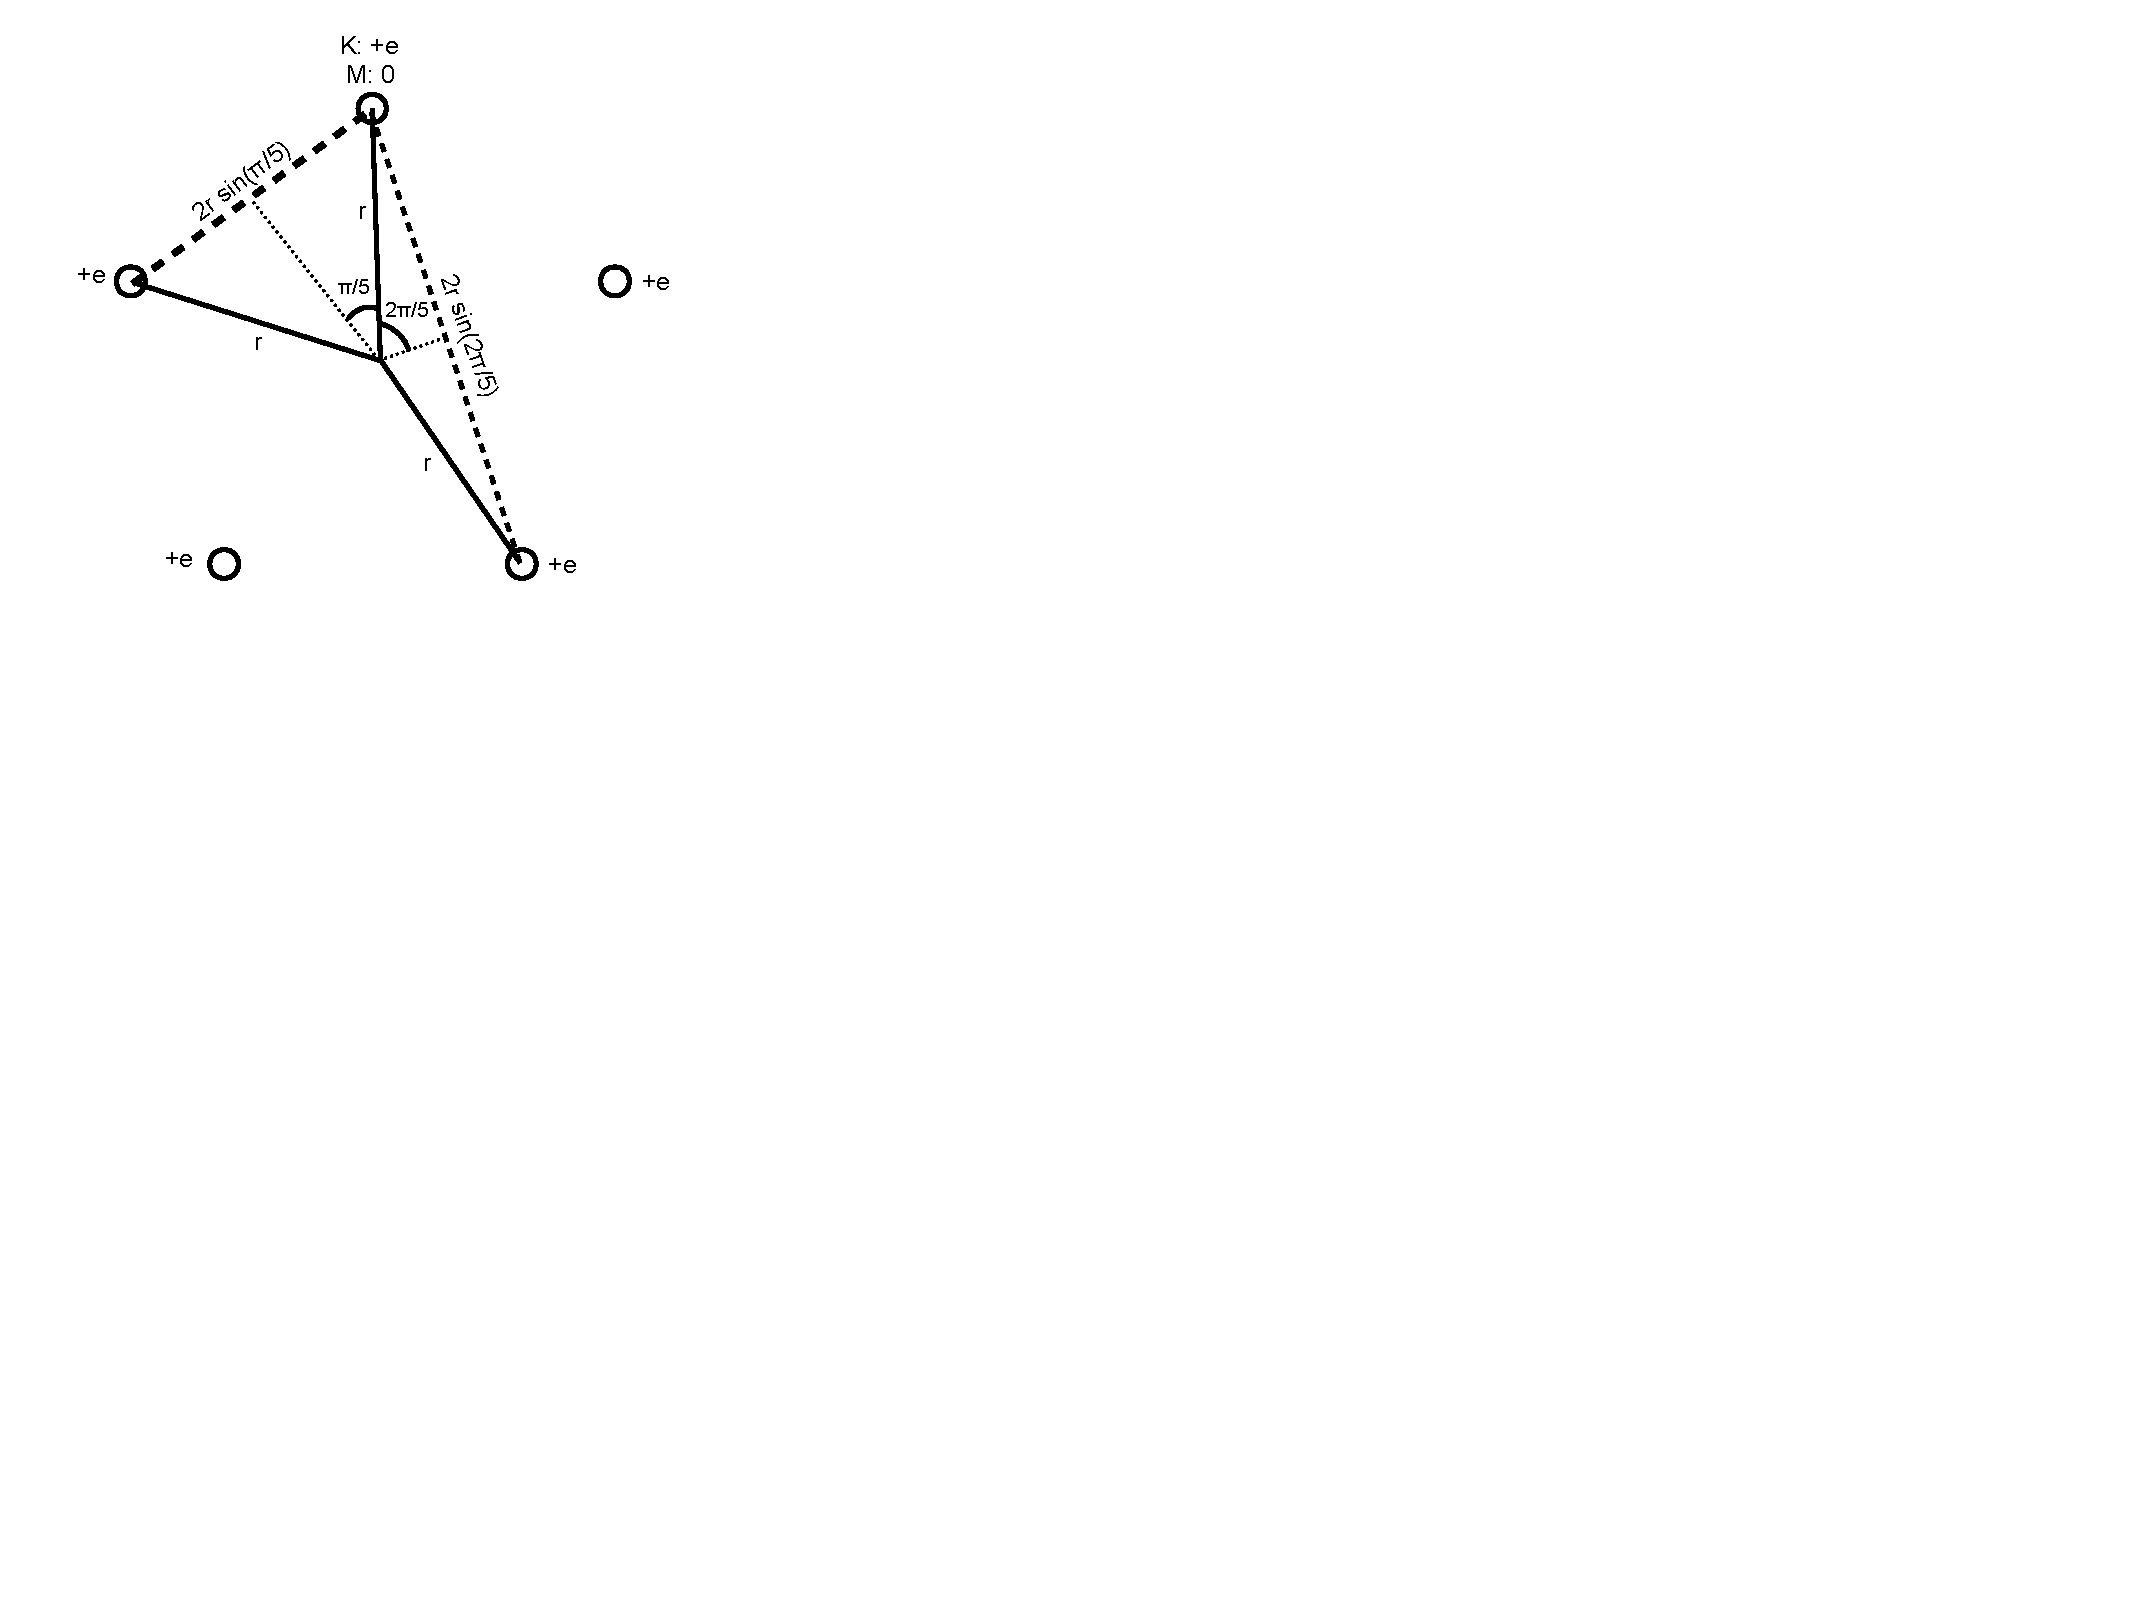
\includegraphics[height=2.5in]{figures/diagram.pdf}
%\hspace{0.5in}
%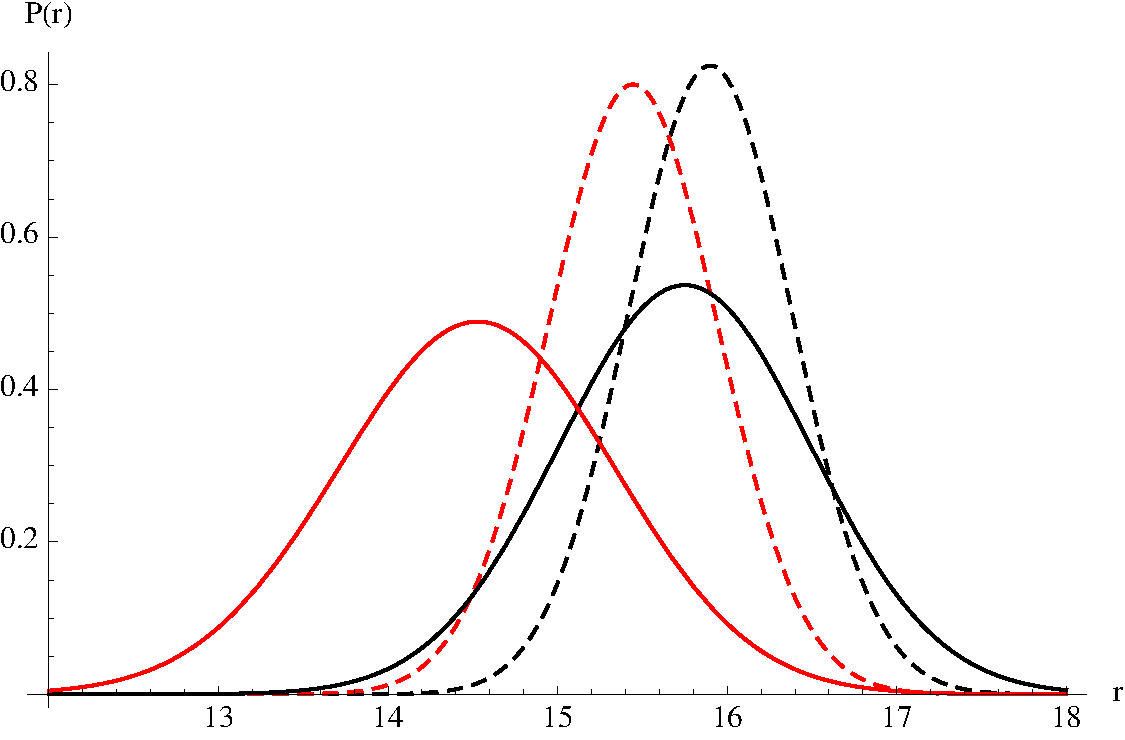
\includegraphics[height=2.2in]{figures/predict_distribution.pdf}
%\caption{A) A conserved basic residue in the M2-M3 loop yields a pentamer of (un-screened) positive charges, which we refer to as the \fiveringnos,  corresponding to $\gamma$ K289, $\alpha$ K279, or $\beta$ K274.  The total energy of the \fivering increases as the ring closes (and $r$ gets smaller), reducing/increasing the distance/repulsion between like-charges. The $\gamma$ K289M mutation neutralizes one of the charges, yielding a +4 ring, which can shrink with a lowered energetic cost.  B) (Placeholder) Predicted distribution  of $r$ generated using values in Table \ref{tab:prediction}; black is for a \fivering (as in K289) while red is for a +4 ring (as in M289); dashed lines are for 300K and solid lines for 315 K.  
%\label{fig:diagram}}
%\end{center}
%\end{figure}

 %\section*{THEORY\label{sec:theory}}
\subsection{Analytical Prediction of Multibody Interactions\label{sec:theory}}
Our simulation analysis is motivated by the multibody interactions within two arrangements of charges found around the GABA(A)r pore, representing the \fivering and the \triadns. 
Each arrangement includes residues on opposite sides of the pore, and the plane containing the residues is normal to the pore axis, so attractive and repulsive interactions within the arrangement will contribute directly to pore-closing and pore-opening, respectively. % almost 100\% of the interactions between them will be directed along the plane of the pore, serving to open or close it. 

\subsubsection*{Charged pentamer}
\newcommand{\side}{r}
\newcommand{\diag}{s}
\newcommand{\avgside}{\bar{\side}}
\newcommand{\avgdiag}{\bar{\diag}}
\newcommand{\avgsidevar}{\bar{\delta\side}^{2}}
\newcommand{\avgdiagvar}{\bar{\delta\diag}^{2}}

As shown in SI Theory, the total Coulomb energy for a charged pentagon with average side length $\avgside$ and average diagonal length $\avgdiag $ is 
%%%
%%%For simplicity, we consider two possible conformations of the pentamer containing these 5 charges : Regular, which has exact five-fold symmetry with 5 sides of length $r_{1}$, and elongated, which has three sides of length $r_{1}$ and two adjacent sides of length $r_{2}$, with only two-fold symmetry.  The total Coulomb energy is given by
%\begin{equation}
%U_{+5} = \frac{ 5 k_{e} e^{2}}{\avgside}
%\left( 1+  \frac{\avgside}{\avgdiag}\right) + O(\avgsidevar)+ O(\avgdiagvar)
% \label{eq:prepentamer}
%\end{equation} 
\begin{eqnarray}
U_{+5}(\avgside, \delta_{\phi}) = \frac{ 5 k_{e} e^{2}\phi}{\avgside}\left( 1+ \frac{\delta_{\phi}}{\phi} \right) + O(\avgsidevar)+ O(\avgdiagvar)
 \label{eq:pentamer}
\end{eqnarray} 
where $e$ is the electron charge, $k_{e} = 332 \mathrm{\AA/kcal/mol}/e^{2}$ is the Coulomb constant, and $\avgsidevar$ and $\avgdiagvar$ are the variance in $\side$ and $\diag$ across the five sides of the pentamer.  For a regular pentamer $\avgdiag = \phi\avgside$ where $\phi \equiv \left(1 + \sqrt{5}\right)/2\sim 1.62$ is a geometric constant often called the ``golden ratio'', with the convenient property $1/\phi = \phi - 1=0.62$.  
$\delta_{\phi}$ is the deviation of $\frac{\avgside}{\avgdiag}$ from the value for a regular pentamer :  $ {\delta_{\phi}}\equiv \frac{\avgside}{\avgdiag} -(\phi - 1)$.

\begin{figure}[t]
\begin{center}
%\centering
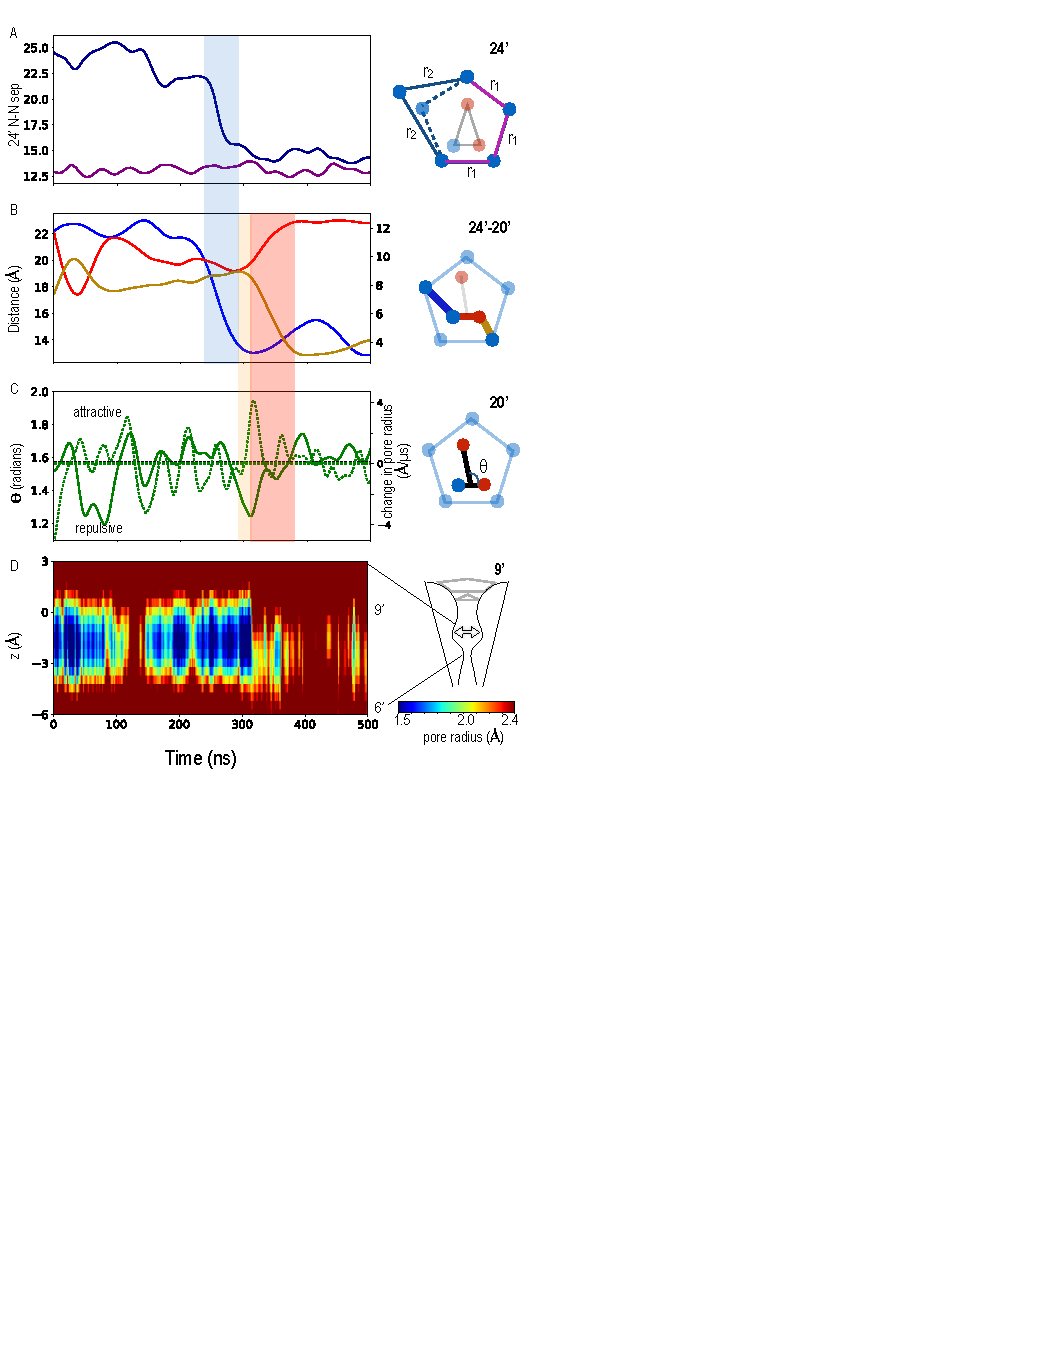
\includegraphics[height = 4in]{figures_2/cartoon_theory.pdf}
\caption{{\bf Evolution of the \fivering and \triad in one replica of the \WT system at 315K.} (A) Flip of one residue ($\alpha$-K279) so the \fivering switches from elongated to regular pentamer, occurs at $\sim$250 ns, followed by a series of events leading to the pore opening between $\sim$250 ns - 350ns, as marked by the shaded regions. (B) The distances between residues $\alpha$K279 -- $\gamma$K285, plotted on y-axis and  $\gamma$K285 -- $\beta$-K270, $\beta$-K270 -- $\beta$-K274, plotted on alternate y-axis, are shown in blue, red and gold respectively. (C) The solid green curve depicts the angle between the charge-dipole arrangement representing the \triad; The Dotted green line represents the pore-opening event as measured by calculating the  first derivative of the minimum pore radius. (D) Pore radius as a function of distance along the pore axis and time.  All curves are smoothed as described in SI Methods.  Transition windows are shaded blue (early), orange (mid), and red (late).   }
\label{fig:theory}
\end{center}
\end{figure}

The linear term in $\delta_{\phi}$ reflects the effects of shape fluctuations on the relative contributions of diagonal and adjacent pairs.   Second-order terms given by $\avgsidevar$ and $\avgdiagvar$ reflect variance in the adjacent and diagonal distances respectively.  According to Eq. \ref{eq:pentamer}, positive values of $\delta_{\phi}$ (in which diagonal distances are shorter than expected in a regular pentamer) will increase the overall energy of the \fiveringnos, provided the average distance between adjacent residues ($\avgside$) is kept constant.  This asymmetry-induced increase in energy can be offset by an overall increase in the size of the \fivering: $\delta_{\phi}$ >0  will stabilize a larger $\avgside$.  Similarly, negative $\delta_{\phi}$ will decrease the overall energy of the \fivering and allow it to close with reduced penalty.  

% $\rho \equiv {r_{1}}/{r_{2}}$ is the ratio of the side lengths and is unity for a regular polygon.  
%%%$\phi \equiv \left(1 + \sqrt{5}\right)/2\sim 1.62$ is a geometric constant usually called the ``golden ratio'', representing the ratio between the lengths of a pentagon diagonal and side, and with the convenient property $1/\phi = \phi - 1=0.62$. Then $g(\frac{r_{1}}{r_{2}})$ is the contribution from deviation from a regular shape, such that $g(1) = 0$:
%%%\begin{eqnarray}
%%%%U_{ring} &=& \frac{ k_{e} e^{2}}{r_{1}}\left(3{\phi}+g\left(\frac{r_{1}}{r_{2}}\right)\right)\\
%%%%\frac{4}{\sqrt{5 + 4((\frac{r_{2}}{r_{1}})^{2}-1)(\phi+2)}}\right)
%%%%\mathrm{(elongated)}\\
%%%%U_{ring} &=& \frac{ 5 k_{e} e^{2}\phi}{r_{1}}\left(1+g\left(\rho\right)\right)\\%\frac{4}{\sqrt{5 + 4((\frac{r_{2}}{r_{1}})^{2}-1)(\phi+2)}}\right)
%%%%\mathrm{(elongated)}\\
%%%%\frac{4  }{  g},
%%%%\frac{2 (2 \alpha +g)}{\alpha  g \text{r1}}+\frac{3 \phi }{\text{r1}}
%%%		%&=&  \frac{ k_{e} e^{2}}{r_{1}}\left(5{\phi}\right),\mathrm{(regular)}\\ %\frac{5 c (\phi +1)}{r \phi }
%%%%		5 \phi g(x)&\equiv&{2}{x} \left(1+\frac{1}{\sqrt{1+\frac{x ^2}{2 }+
%%%%		\frac{1}{x}  \sqrt{(1+\phi^{2} )\left(1-\frac{\phi^{2}x ^2}{4}\right)}}
%%%%		}\right) - 2\phi \\
%%%		g(x)&\equiv&-\frac{2}{5}+\frac{2}{5} \frac{x }{\phi }\left ( 1
%%%		%\frac{2}{5} \left(\frac{\rho}{\phi} -1\right) 
%%%		+ \frac{1}{  \sqrt{1+\frac{x ^2}{2 }+
%%%		\frac{1}{x}  \sqrt{(1+\phi^{2} )\left(1-\frac{\phi^{2}x ^2}{4}\right)}}
%%%		} \right)\\
%%%		&=& \left(1 - \frac{2}{5 x}\right) \frac{(x - 1)}{x} + O((x-1)^{2})
%%%		%\frac{2}{\rho}\left(1 + \frac{1}{2\sqrt{ 1+\frac{1}{2 \rho^{2}}+ 2\sqrt{(\phi +2) \left(1-\frac{\phi^2}{4\rho^{2}}\right)} }}\right)\\
%%%		\end{eqnarray}
%%% (further details in SI Methods).  %Check coefficients - should be more \phi?
%%%
Neutralizing any of the charges removes two diagonal and two adjacent interactions, so the Coulomb energy for 4 like-charges arranged on a pentagonal lattice is
\begin{eqnarray}
U_{+4}(\avgside,\delta_{\phi}) &=& \frac{ 3 k_{e} e^{2}\phi}{\avgside}\left( 1+ \frac{\delta_{\phi}}{\phi} \right) + O(\avgsidevar)+ O(\avgdiagvar)\\
& =& \frac{3}{5} U_{+5}(\avgside,\delta_{\phi})
 \label{eq:mutant_pentamer}
\end{eqnarray} 
where averages only consider distances involving charged residues, and therefore $\avgside$ and $\delta_{\phi}$ incorporate only three adjacent distances and three diagonal distances.  The factor of 3/5 will generally stabilize a smaller value of $\avgside$ at any temperature, but $\delta_{\phi}, \avgsidevar, \avgdiagvar$ will also be directly dependent on temperature. 
%%%\begin{eqnarray}
%%%U_{+4}(r_{1},r_{1})= \frac{ 3 k_{e} e^{2}\phi}{r_{1}} = \frac{3}{5} U_{+5}(r_{1},r_{1})
%%%\end{eqnarray}
%%%and all forces or other derivatives will be also be equivalent to 3/5 multiplied by their value in the fully charged pentamer. 
%%%
%Unless stated otherwise, any claims regarding configurational energies for the \fivering are based on these equations.  
The simple Coulomb calculation represented in Eq. \ref{eq:pentamer} indicates a large energetic cost of shrinking the \fiveringnos over typical distances (Fig \sFigEnergy B).  Considering typical distances between homologous residues in \plgics, the strength of the interaction among homologous residues may be unintuitive.  %  residues that  separations  the size of the \fivering $r_{1}$ may be unintuitive, especially for large values of $r_{1}$ . 
Reducing the distance between two like charges from $r_{1}=15\AA$ to $r_{1}=12\AA$ raises the electrostatic energy by only 5.5 kcal/mol, but shrinking the regular pentagon (including diagonal interactions) from $r_{1}=15\AA$ to $r_{1}=12\AA$ increases the energy of the arrangement by 49 kcal/mol!  Diagonal, cross-pore interactions contribute almost 20 kcal/mol, nearly doubling the total.  
\subsubsection*{Charge-dipole}

Farther away from the interface with the ECD, facing the pore, is another charged ring of three residues, at M2 20$^{\prime}$ ($\beta$E270 and $\gamma$K285), that we term the ``\triad'' because it exhibits rapid shape fluctuations that are propagated to the hydrophobic gate.  The Coulomb energy reflects two diagonal interactions, and one adjacent interaction, and is effectively a charge-dipole interaction: % (although the common approximation that the separation $r$ between the dipole midpoint and the charge is much longer than the separation of two charges within the dipole $d$ does not hold).  %Shape fluctuations are much more common in this triang than the +5 pentamer, and we relax the requirement of a regular polygon.  
%The Coulomb energy is 
%\begin{equation}
%U_{c-dp} = -{ \frac{k_{e} e^{2}}{r}}\left(-\frac{1}{\sigma} + \frac{1}{\sqrt{{1+\frac{\sigma^{2}}{4} +   \sigma \cos \theta }}} 
%+ \frac{1}{\sqrt{{1+\frac{\sigma^{2}}{4} -   \sigma \cos \theta }}} \right) 
%%  \sigma \equiv d/r
%\end{equation}
\begin{eqnarray}
U_{c-dp} &=&- { \frac{k_{e} e^{2}}{r}}\left(\frac{r}{d} + \frac{1}{z^{+}} 
- \frac{1}{z^{-}}\right)\label{eq:triad} \\ 
  z^{\pm}&\equiv&\sqrt{{1+\left(\frac{d}{2 r}\right)^{2} \pm  \frac{ d\cos \theta}{r} }}
%  \sigma \equiv d/r
%U_{coul,+1} &=& { k_{e} e^{2}}\left(-\frac{1}{r_{1}} - \frac{1}{r_{2}} + \frac{1}{r_{3}}\right)\\
%&=&\frac{1-\sin \theta _3\left(\csc \theta _2+\csc \left(\theta _2+\theta _3\right)\right)}
%{\sqrt{A~{\sin\theta _3} ~{\csc \theta _2} ~{\csc \left(\theta _2+\theta _3\right)}}}
\end{eqnarray}
where $U_{c-dp}$ is the Coulomb energy of the charge-dipole, $d$ is the distance between the two charges forming the dipole, $r$ is the separation between the charge and dipole midpoint, $z^{\pm}$ are the distances between the charge and the close and far ends of the dipole, respectively, and $\theta$ is the angle between the dipole and dipole midpoint-charge separation vector (see diagrams in Fig. \ref{fig:Pillar_2_graphs_network}C and \sFigEnergy B). 

It is common in undergraduate-level treatment of charge-dipole interactions to assume $r/d>> 1$ in Eq. \ref{eq:triad}, but for a charge-dipole arranged on a regular pentagonal lattice,  $r/d \equiv \phi \sim1.6$.  One central result from the usual treatment is that at $\theta = \pi/2$, the interaction switches from being attractive to repulsive, with a discontinuity at the boundary; this result still holds in the full expression (Fig \sFigEnergy B), 
as expected.  
%The full  expression has some additional dependence on $\theta$, which becomes pronounced at small values of $r/d$.  

%\begin{table}[htpb]
%\caption{Change $\Delta U$ in net electrostatic energy of a charged pentamer upon a decrease in the average side distance $\avgside$ from 15$\AA$ to 12$\AA$ (as observed in the spontaneous opening in Fig \ref{fig:theory} A), calculated using Eq \ref{eq:pentamer} for the pentamer with charge +5 and Eq \ref{eq:mutant_pentamer} for the pentamer with charge +4.  \grace{This table could probably be removed}}
%\begin{center}
%\begin{tabular}{|c|c|c|}
%$\delta_{\phi}$ & $\Delta U_{+5}$ (kcal/mol) & $\Delta U_{+4}$ (kcal/mol)\\
%\hline
%%Reducing separation of single pair from $r_{1}=15\rightarrow12\AA$ & 5.5 \\
% 0.1&48 & 29\\
% 0& 45 & 27\\
% -0.1 & 42 & 25\\ 
%%Adjacent Contribution & 28 \\
%%Diagonal Contribution & 17 \\
%%Elongated to Regular; 
%%15 &$20\rightarrow 15$ &5 & 11& 7 & 4 \\
%%%15 &$20\rightarrow 15$ &4 & -& - & - \\
%%15& 15& 5$\rightarrow$4 & -90 & -56 & -34\\
%\end{tabular}
%\end{center}
%\label{default}
%\end{table}% 

\section*{RESULTS AND DISCUSSION}
%Rework to refer to table

%More generally, the coulomb interaction between two charges placed on the diagonal of a regular pentagon will only be moderately reduced from the interaction they would have as adjacent charges. The diagonal contribution to the electrostatic energy is just the adjacent contribution divided by $\phi$, and because a charge on a pentagon has an equal number of diagonal and adjacent interactions, diagonal interactions will contribute $1/(1 + \phi) = 38\%$ of the overall interaction energy.  This result holds regardless of the distance of the charges (or residues) from the pentagon (or pore) center, but does require pentameric symmetry. In any particular \plgic , we can conclude that {\emph {any} charged residues conserved across subunits} will contribute to stabilizing an open pore.  Such residues may be in the M1 linker in some heteromeric \plgics (like \nachr) and in the M2-M3 loop in other heteromeric \plgics (such as \GABAA).  Any charged residue in a homomeric pLGIC will have this property at a pH for which nearly all of the residues are charged.  %; in this case, sensitivity may be significantly reduced by an adjacent residue of opposite charge, which converts the arrangement of five like charges into an arrangement of five dipoles
%Eq. \ref{eq:triad} yields an attractive charge-dipole interaction that favors reducing $r$ when $\theta < \pi/2$, and a repulsive interaction that favors increasing $r$ when $\theta > \pi/2$; there is a discontinuity at $\pi/2$.  As a result, a charge-dipole configuration may oscillate at high frequency if localized around $\theta\sim\pi/2$, indicating a potential role for single-channel flickering, allosteric gating, and rapid signaling in GABAA receptors.  

\subsection*{Spontaneous opening event at 315 K}
%TEMP
A spontaneous opening event was observed in one \WT replica at the higher temperature.  In this replica, the pore was closed for over 500~ns at 300K (Figure \SklowTrepTwo), but after raising the temperature to 315K and about 200~ns of simulation, a spontaneous set of events induced a stable open pore for the remainder of the simulation.  (Figure \ref{fig:Pillar_2_graphs_network}, and SI Movie \SkMovie).   The event itself took about 100-150 ns, and involved the following stages, shaded by the specified colors in Figure \ref{fig:Pillar_2_graphs_network}.

\begin{figure}[t]
\begin{center}
%\centering
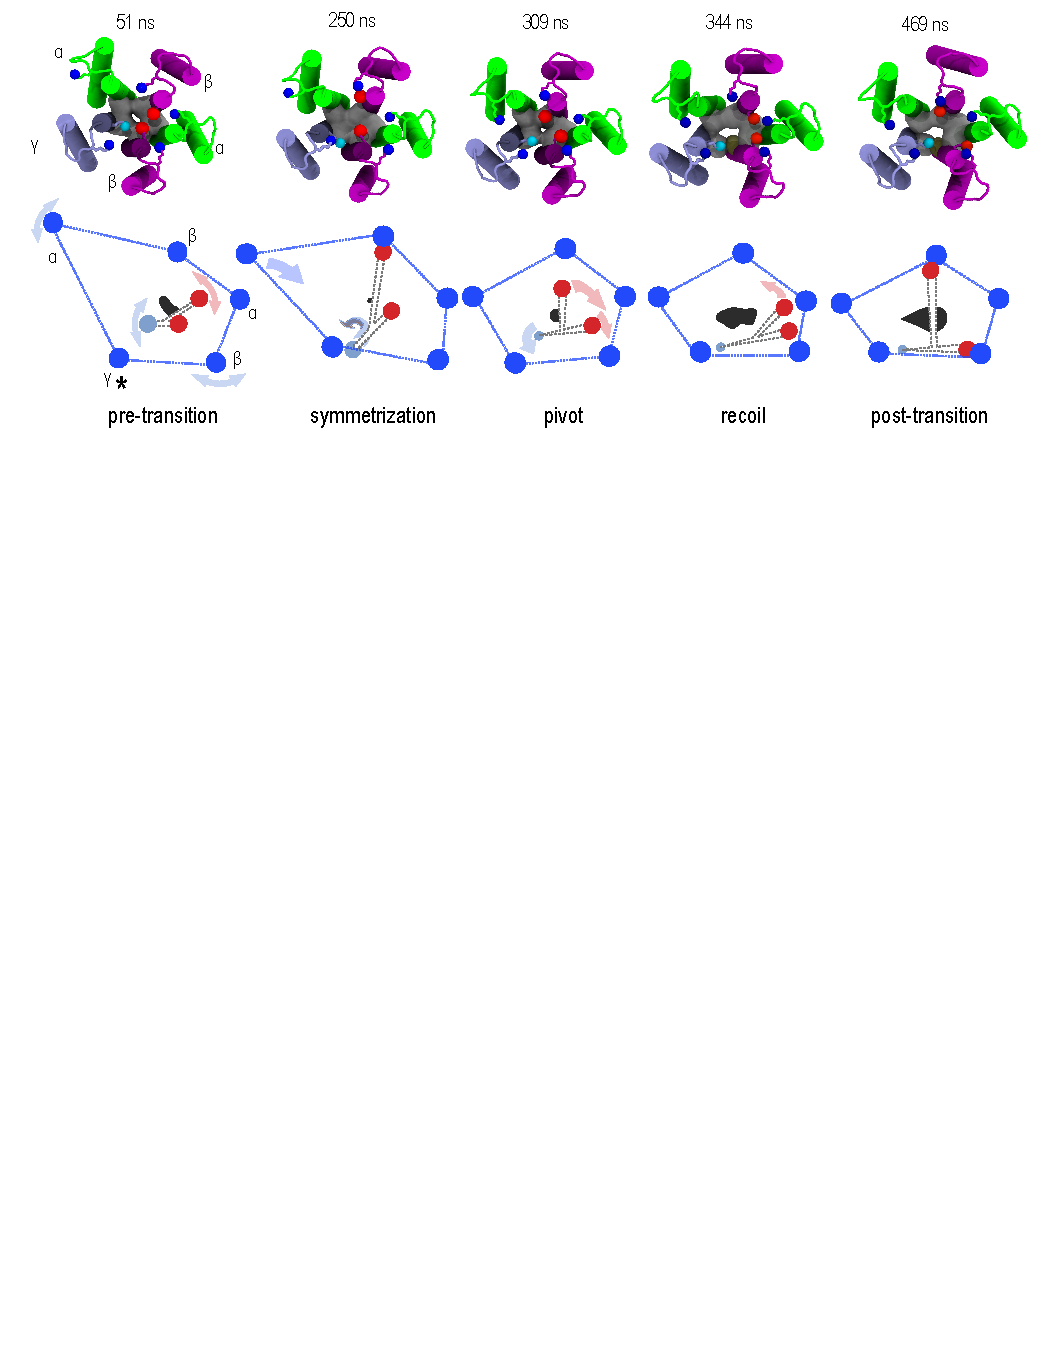
\includegraphics[width =0.5\textwidth]{figures_2/Cartoonv4}
\end{center}
\caption{{\bf Evolution of \triad and \fivering during spontaneous opening event.} Top: Representative frames are shown from the \WT trajectory at 315K, with coloring as in Figure 1B/C. Bottom: Cartoon of transition highlighting movement of the charged groups forming \fiveringnos (blue) and \triad ($\gamma$K280-cyan, $\beta$E270-red).  Dashed lines connecting the points of the \triad and \fivering are for visualization purposes only and do not represent physical bonds. The filled gray shape indicates the unoccluded area of the hydrophobic gate. After $\alpha$ K279 flips during the symmetrization step, M2 helices separate along the axis connecting the flipped and current positions (frame at 344 ns), while after the acidic residues pivot, M2 helices separate along the axis connecting the two acidic residues (post-transition panel). Salt-bridges are represented by contacting red and blue spheres. The asterisk marks the charge that is neutralized with the K289M mutation.} 
\label{fig:Pillar_2_graphs_network}
\end{figure}
%\begin{figure}[htp]
%\begin{center}
%%\centering
%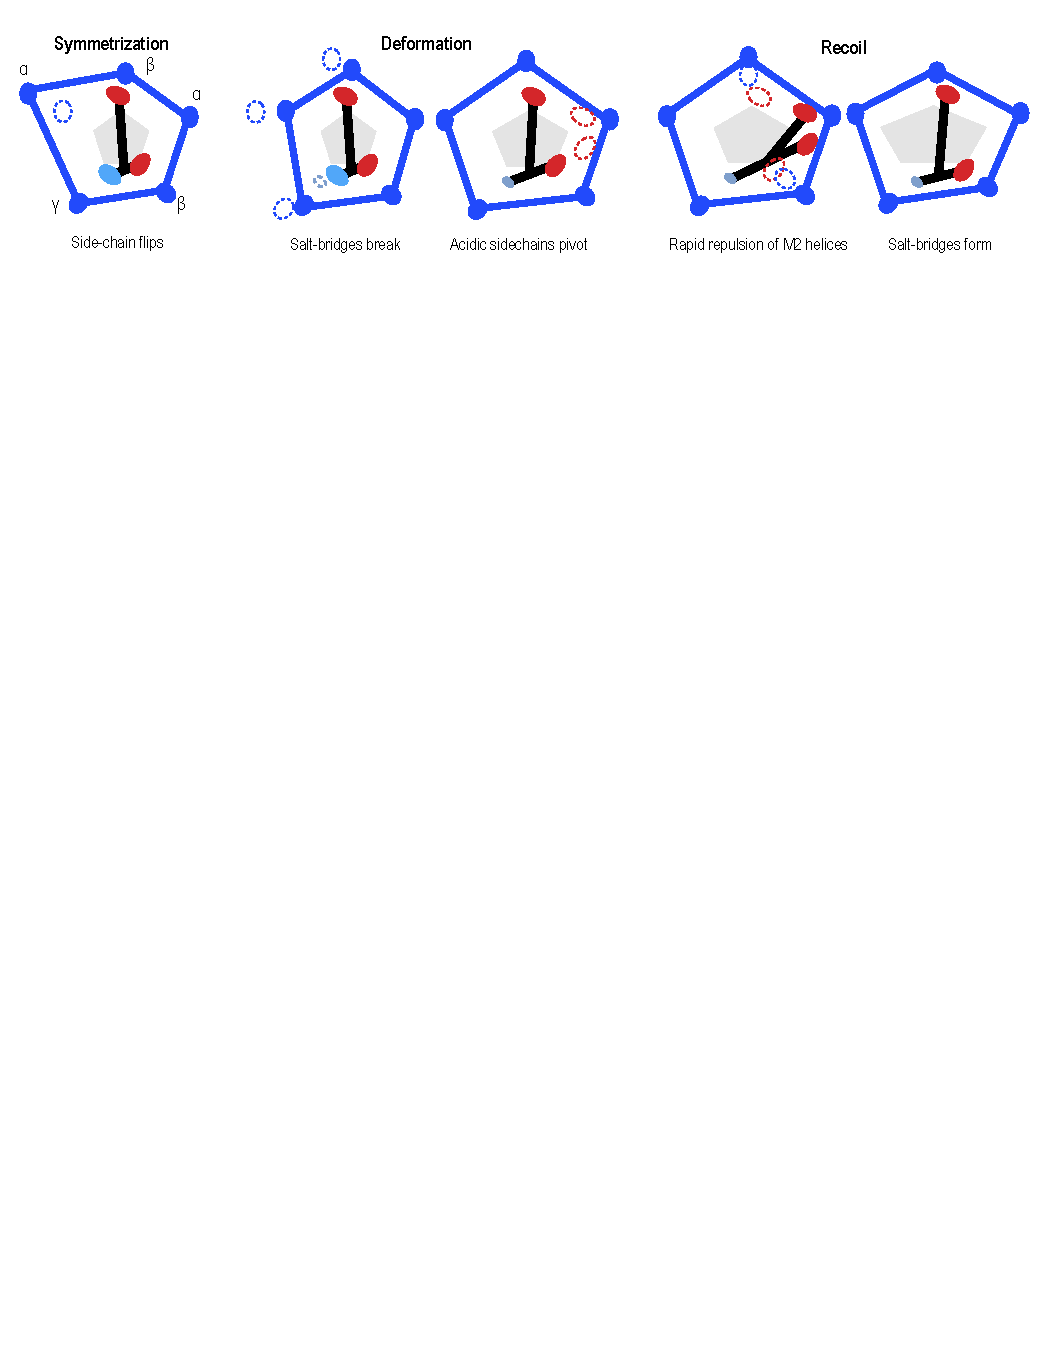
\includegraphics[width = 0.5\textwidth]{figures_2/Cartoonv3.pdf}
%\caption{\label{fig:finalcartoon} Cartoon of observed stable spontaneous opening event %and analogous process in $\gamma$K289M mutant receptors, 
%with associated transitions. Interfacial band is shown with positively charged sidechains in blue; \triad is shown with positively charged and negatively charged sidechains in cyan and red, respectively.  Future positions are noted by a dashed outline. Relative shape and size of the minimum pore constriction is illustrated using a filled gray pentamer. The cation in the \WT \triad is deflected toward the intercellular domain upon flip, illustrated by the shrinking cyan shape; this step is missing in the $\gamma_{2}$K289M mutation, which neutralizes one the $\gamma_{2}$ charge in the \fiveringnos. \grace{We should maybe combine this with Figure 3. }}
%\end{center}
%\end{figure}

\begin{enumerate}
\item {\bf Early  (blue): Symmetrization of \fiveringnos.} The \fivering begins in an elongated conformation, because the side-chain of one charged residue ($\alpha_{\gamma}$-K279) faces away from the pore axis, while all other side-chains face toward it. Between 200 and 260~ns, this side-chain flips, causing the \fivering to switch from an \extended to a regular conformation (Figure \ref{fig:theory} A).  This flip may be dependent upon flexibility introduced by the adjacent proline ($\alpha$P278); the conservation\cite{Jaiteh2016} and significance of this proline for function\cite{Lummis2005} are well-established, although its fundamental role in gating has been unclear. % .  A slight raise in temperature was sufficient to cause the flip in an unliganded receptor over simulation time-scales; the likelihood that binding of a ligand reduces the energetic penalty of this conformational change is strong and considered in the discussion.  
  %These simulations suggest its role may be in facilitating the rapid switch of charged side-chains M2 24$^{\prime}$ between facing away from the pore and facing in toward the pore.  
\item {\bf Mid  (orange): Response to symmetrization; partial opening and deformation.}
\begin{enumerate}
\item t = 260-300 ns: The previous symmetrization step is electrostatically unfavorable for the other residues of the \fivering and for the basic residue of the \triadns; in response,  the M2 helices of the flipped $\alpha$ subunit and the $\gamma$ and $\beta$ subunit on either side separate from the other two subunits. This initiates widening of the pore, as shown by the sharp transition in Figure \ref{fig:theory} D.   Simultaneously, the positively-charged end of the \triad dipole ($\gamma$-K285) is deflected toward the intracellular domain and away from the ECD (Figure \ref{fig:Pillar_2_graphs_network}). This destabilizes its salt-bridge with the negatively charged residue comprising the other end of the ``dipole'', $\beta_{\gamma}$-E270.  

\item  t=300-330~ns: Upon weakening of favorable electrostatic interactions with positively charged residues in the \triad and \fiveringnos,  the two negative sidechains of the \triad pivot around their $C_{\alpha}$ atom to face away from the $\gamma$ subunit.  This switches the \triad charge-dipole interaction from attractive to repulsive, as tracked by $\theta$ in Figure \ref{fig:Pillar_2_graphs_network} C and according to Eq.  \ref{eq:triad}; for small values of $\theta$, the distance between the two negatively charged residues becomes particularly small (Figure  \ref{fig:Pillar_2_graphs_network}). % The charge-dipole interaction is attractive for $\theta > \pi/2$ and repulsive for  $\theta << \pi/2$ (Eq. \ref{eq:triad}).  %The \triad  The cross-pore interaction between the charge and dipole of the \triad switches from attractive to repulsive as $\theta$ becomes less than $\pi/2$, leading to rapid shape and scale oscillations (Eq. \ref{eq:triad}).  
%Due to the discontinuity, rapid fluctuations in the pore-oscillator are significant at both 300K and 315K, and periodically these fluctuations result in a very small value of $\theta$.  %corresponding to the two negatively-charged side chains of the \triad becoming close, which 
%This occurs twice in this particular trajectory (once at $t=100~ns$ and once at $t=350~ns$). 
\end{enumerate}

\item {\bf Late (red): Recoil and Stabilization.} 

The pore-oscillator is now in a highly unfavorable configuration due to proximity of the two negative charges corresponding to low values of $\theta$.  %indicated in Figure \ref{fig:theory}C by the very low value of $\theta$ at $t\sim 325~ns$).  
The resulting repulsion causes a rapid separation of the charges. This is further propagated to increase the distance between their respective M2 helices, as indicated by an additional increase in pore radius, not just %entire pore profile. (Figure \ref{fig:theory} C \& D). As a result, the strong repulsion directly precedes a rapid opening of the pore, not just 
at the \triad but also at the minimum constriction 16-17 Angstroms away  (Figure \ref{fig:theory} D). 
The trajectories of $\theta$ and the time derivative of the minimum pore constriction are shown plotted on the same axis in Figure \ref{fig:theory} C; the two most rapid increases in the pore radius each occur directly after the two $\theta$ compression events (at t = 100~ns and t = 325~ns).  This association was also qualitatively observed in the other replica trajectories (Figures \sFigReplicas), although in some cases it was a less acute value of $\theta$, held over a longer time period, that preceded opening.  

Upon recoil, each of these two acidic residues formed an intrasubunit salt-bridge with a basic residue of the \fivering (Figure \ref{fig:theory} B). Since the charged \fivering is resistant to shrinking, these salt-bridges can only form if the acidic residues in the \triad are also separated. The timing of events is consistent with \triad recoil simultaneously allowing salt-bridging with the \fivering and causing an overall separation of M2 helices. Due to the stochastic nature of the trajectory, determining the typical order of these two events would require many more replicas.
%Swapping of salt-bridges in the electrostatic network formed by the \triad and \fivering allows the \triad to salt-bridge with the \fivering at two locations (Figure \ref{fig:theory} B).  
%In the particular replica shown here, this occurs when repulsion between two positively charged residues (the newly flipped $\alpha$-K279 of the interfacial-band and $\gamma$-K285 of the \triad dipole) destabilizes the salt-bridge between the two dipole residues ($\gamma$-K285 and $\beta_{\gamma}$-E270). $\beta_{\gamma}$-E270 can then form a new salt-bridge with another \fivering residue ($\beta$-K274).  
\end{enumerate}
  %\item {\bf t=370~ns: Pore opening} Opening of the pore at the hydrophobic gate is extremely rapid following compression (within ns)  (Fig. \ref{fig:Pillar_2_graphs_network}) 
The \triad samples small values of $\theta$ regardless of the configuration of the \fiveringnos, due to high frequency oscillations consistent with the discontinuity in the interaction, including twice in this particular trajectory (once at $t=100~ns$ and once at $t=350~ns$). Such events were observed in all simulated systems and were usually followed by brief opening of the pore. A stable opening event, however, was only observed when salt-bridging of each of the pairs of $\beta$-E270 and $\beta$-K274 residues was also stable, which depended upon the symmetrization step.  % was highly correlated with an open pore in other trajectories and temperatures, but these were  short-lived for short-lived latched states (Figure\ref{fig:Pillar_2_graphs_network}).  
%In this state, the positively charged side-chains of the \fivering face the center of the pore, increasing their repulsion with the rest of the \fiveringnos, and stabilizing a symmetric \fivering and open pore.  
The significance of the symmetric \fivering is verified through the next set of simulations involving a mutant of an \fivering residue.  
%In summary, swinging the anion of the \triad toward the anionic end of the \triad dipole causes rapid separation of the M2 helices, directly proceeding pore-opening.  Flip of the \fivering from an extended to regular pentagon switches contacts of the electrostatic network and stabilizes the open state, while also reducing pore oscillations.   
%SRUTHI - legends need proper gammas (lower case not uppercase) 
\begin{figure}[t]
%\begin{center}
\centering
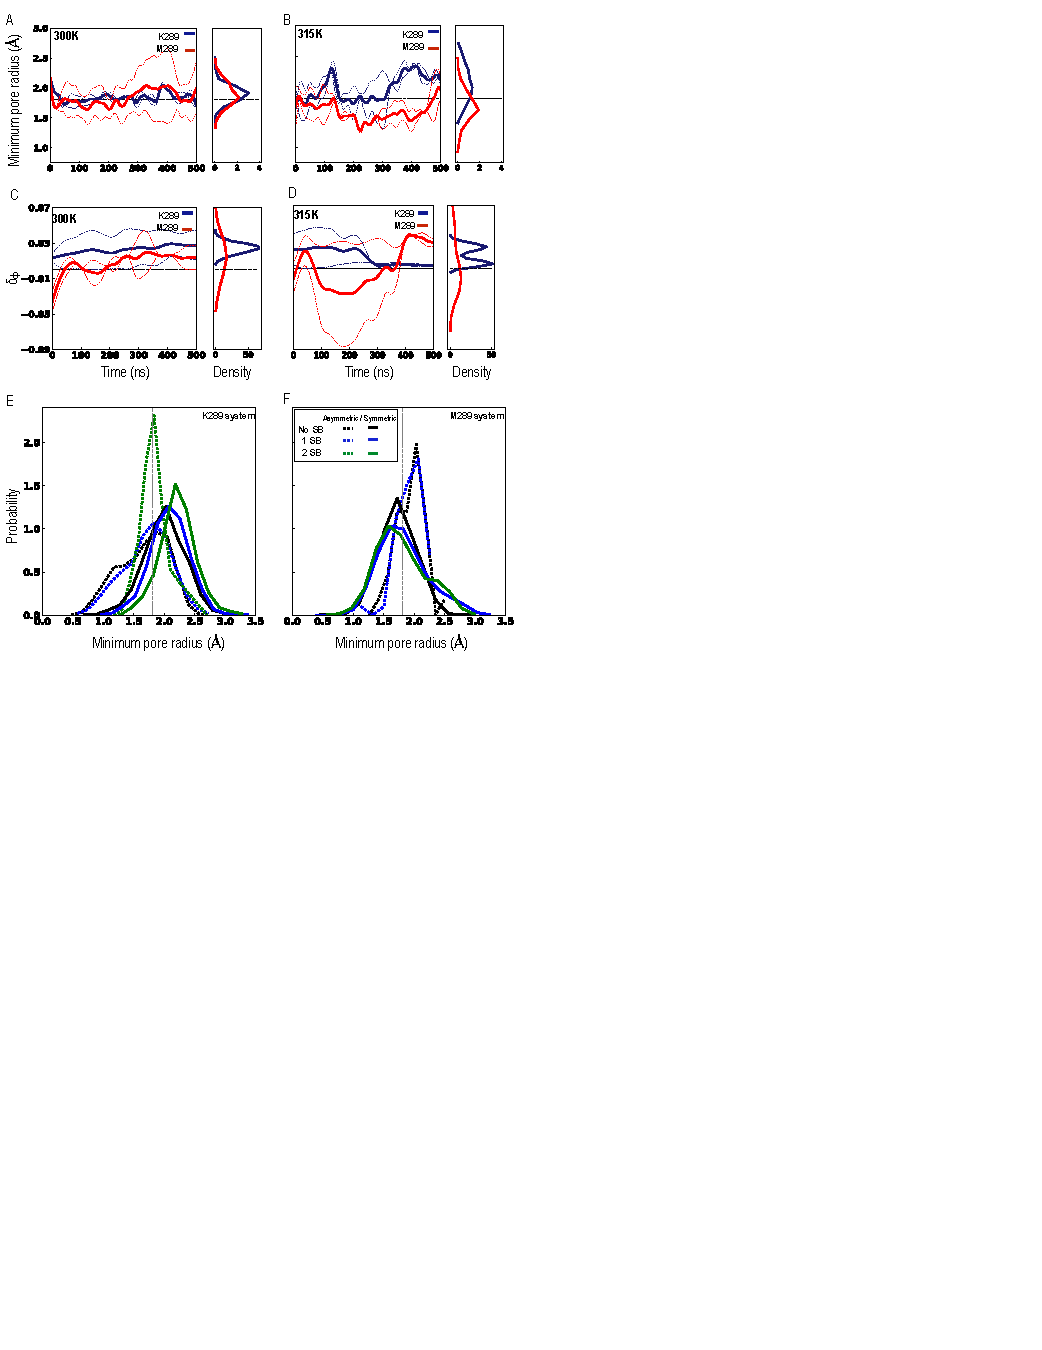
\includegraphics[height = 3.5in]{figures_2/Pillar_4_fig}
%\end{center}
\caption{Correlations between shape of \fiveringnos, pore radius, and salt-bridging between \fivering and \triad for multiple replicas and temperatures.  (A/B) Smoothed time evolution of the pore minimum constriction, averaged (solid lines) over two replicas (shown separately as dotted lines) each, at 300 K and 315 K. 
%The minimum constriction formed around the 9' region is visibly more constricted for the \MTs and this reduction is more pronounced at higher temperature. The minimum constriction region in \MT falls below 
The radius of a chloride ion is represented by the dashed horizontal line at 1.8\AA. 
%The probability distribution further shows a clear shift in the peak of the \MTs towards reduced pore radii at a higher temperature.
(C/D) Smoothed time evolution and distribution of $\delta_{\phi}$ for both \WT and \MT systems at 300 and 315K. Distribution trends are similar to those generated numerically, discussed in SI Theory.  %  in WT in comparison with the Diagonal/Adjacent Ratio of the +4 charges in K289M mutant system at 300 K(C) and 315 K(D). %Higher temperature brings the +5 pentagon Diagonal/Adjacent ratio closer to 
%The expected symmetric value, 1/$\phi$ (dashed line). 
(E/F) Distribution of minimum constriction radius for conformations clustered by total number of $\beta$ K274-E270 salt-bridges and symmetrization of the \fiveringnos. }%While the formation of two salt-bridges following the occurrence of the flip stabilizes the open state of the \WTs , symmetrization and the two salt-bridges do not occur simultaneously in the \MT systems.  }
\label{fig:Pillar_3_fig}
\end{figure}
\subsection*{$\gamma$ K289M increases energetic sensitivity to shape fluctuations of the \fiveringnos} The multibody mechanism proposed in the previous section suggests an important role for each basic residue in the \fivering for conferring stability of the open state, beyond communication with the agonist-binding domain.  $\gamma$ subunits are not required for functional GABA(A) receptors, and do not participate in the interfaces forming the orthosteric binding sites. % but impact of a symmetric \fivering conformation requires each charge in the \fivering regardless of the other residues on the chain. 
Yet neutralizing the $\gamma$-contributed charge to the \fivering causes flickering in single-channel recordings \cite{Bianchi2002}  and is associated with fever-induced seizures. % breaking the pentameric symmetry of the \fiveringnos. 
%TEMP
%In these systems, the flipping of the elongated pentamer to a regular pentamer $\alpha$ subunit was observed within 10 ns of the simulation start, even at the lower temperature, confirming the importance of each charge in the \fivering for forming the barrier to \flip. After the Flip step, however, no Stabilization step was observed; Movie S{\muthotmovie} provides a straightforward representation.  The flexibility of the interfacial 4-ring becomes much more pronounced at 315K, consistent with the importance of fever for inducing seizure in patients with this mutation.   

\begin{figure}[t]
%\begin{center}
\centering
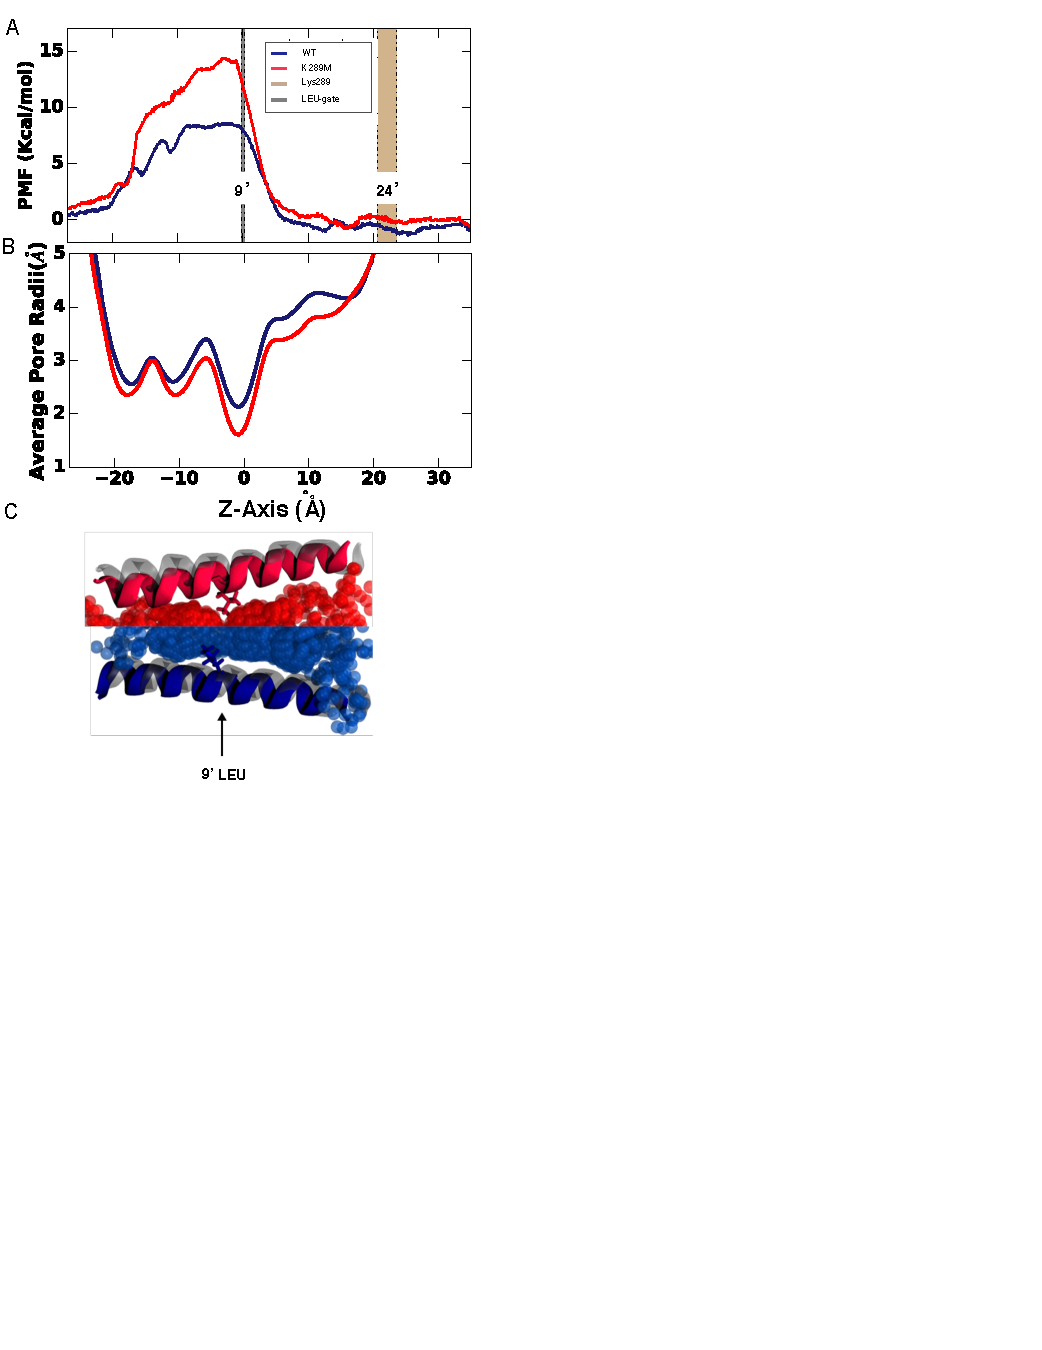
\includegraphics[height = 3in]{figures_2/pillar_4_ABF_2}
\caption{ (A) Potential of mean force profile of a chloride ion crossing the ion channel, calculated at 315K for a receptor that remained primarily in the \extended conformation for the \WT and had a flexible \fivering for the \MT. The full PMF including the rest of the simulation box is in Fig \SFullABF. (B) Average pore radius profile for the conformations in (C).}
\label{fig:abf}\label{fig:pore-profile}
%\end{center}
\end{figure}

Simulations of the two \MT replicas at both 300K and 315K, as for the \WT receptors, indicated a reverse temperature dependence for the distribution of minimum pore radii  (Figure \ref{fig:Pillar_3_fig}).  %pore radii that were consistent with temperature-induced increases in  ramifications of this effect for the pore radius is reflected in the pore radius profile (averaged across time and two replicas) for the \MT and \WT receptors, at both 300 and 315K, shown in Figure \ref{fig:pore-profile}, as well as the trajectories and distributions in Figure \ref{fig:Pillar_3_fig} .  The minimum constriction region occurs at roughly the same height along the pore axis for the two systems %(except for the Latched-open states in the \WT), 
As shown in Figure \ref{fig:Pillar_3_fig} A, we observe no effect of the mutation on the overall distribution of pore radii at 300K.  At 315K, the \WT distribution broadens, as expected (Figure \ref{fig:Pillar_3_fig} B).  The \MT distribution broadens even more at the higher temperature,  but is also shifted toward smaller radii, so that at 315K both \WT replicas have larger pore radii than both \MT replicas for most frames. 

Eq. \ref{eq:mutant_pentamer} indicates three possible contributions to a reduced cost for shrinking the \MT \fivering compared to that of the \WT \fiveringnos: 
\begin{enumerate}
\item The reduced charge of the \MT \fivering results in a factor of 3/5 for the overall energetic cost to shrink the \MT \fiveringnos, assuming the same value of $\avgside$ and $\delta_{\phi}$. This contribution is not temperature dependent, and the 40\% loss is large enough that it is perhaps most surprising that an \MT receptor is functional at any temperature. This may be explained by the observation that in the \MT systems, $\gamma M2 20^{\prime}$ (M2 K285) of the \triad assumes a position much closer to the original position of K289.   
\item  Any reduction in $\delta_{\phi}$ will destabilize the open state by reducing the energetic cost to shrink the \fiveringnos (Eq. \ref{eq:pentamer}).  Both increased temperature and the loss of charge symmetry would be expected to increase the root-mean-square-displacement (RMSD) of each remaining side-chain.  We ran simple numerical calculations to determine how increased RMSD in individual charges affects the distribution of $\delta_{\phi}$, shown in Figure \sfigDeltaPhiDist. The distribution of $\delta_{\phi}$ is not particularly sensitive to RMSD if all five charges of a closed pentagon are used, due to geometric constraints and the non-cohesive nature of the noise. The distribution is expected to widen with increased RMSD, but mainly in the positive direction (Figure \sfigDeltaPhiDist A). 
  \item Even if each individual (conserved) charge has the same RMSD in the \MT and \WT receptors, the distribution of $\delta_{\phi}$ will be broadened in the \MT receptor because only three of the five adjacent and diagonal distances are used to calculate the average adjacent and diagonal distances, and they are not constrained by the requirement of forming a closed pentagon (Figure \sfigDeltaPhiDist). Furthermore, the broadening is symmetric, with significant probability of $\delta_{\phi} < 0$. This is consistent with what we observe in the molecular systems, as shown by  deviations of the ratio of diagonal to adjacent distances from $1/\phi$ (Figure \ref{fig:Pillar_3_fig} C,D) over each trajectory.  
  \end{enumerate}
Comparison between Figure \ref{fig:Pillar_3_fig}A,B and C,D, reveals similar trends for distributions of minimum pore radius and $\delta_{\phi}$, upon introducing the mutation, raising the temperature, or both.   %These results are consistent with a mechanism in which temperature increases shape fluctuations for both the \MT and \WT \fiveringnos, but the overall energy of the \MT \fivering is much more sensitive to the \fivering shape.  

%  increase deviation of the remaining individual charges from a regular pentagonal lattice; this effect may be exacerbated by temperature.  ,\end{enumerate}
%,  The distribution of $\delta_{\phi}$ values, however, is determined by the number of adjacent and diagonal distances used to calculate them. When all charges are on a regular pentagonal lattice (even if not all sites are occupied), $\delta_{\phi} = 0$.  When the charges deviate slightly from these positions, $\delta_{\phi}$ will depend on how many distances are incorporated into the average, as shown in Figure S\ref{fig:avgdist}.   For a small random deviation of any five points, $\delta_{\phi}$ is strongly peaked near 0, with a significant positive tail when five points are used, with a more symmetric, broad distribution predicted when only four points are used.  This affect is enhanced significantly when the allowable random deviation is increased (similar to a rise in temperature), and although $\delta_{\phi}$ assumes still few negative values when all five points are used, it has far significant negative density when only 4 points are used. This prediction indicates that {\emph even if the \fivering charges conserved in both the \MT and \WT receptors had the exact same deviations from pentagonal symmetry, the addition of an additional charge in the \WT case will reduce the overall average deviation. Finally, because of the lack of charge symmetry, it is expected that the overall deviation from a pentagonal lattice will be increased in the case of the \MT receptor.  
%      Neutralizing one charge in the \MT \fivering results in shape changes  
%In these systems, the barrier to \fivering shape changes is much lower; the \fivering rapidly flips to a regular conformation upon the simulation beginning, but this is simply the first of many shape oscillations over the course of the simulation.  

% This shift was correlated to an increase in asymmetry of the \fiveringnos, which was tracked via deviations of the ratio of diagonal to adjacent distances from $1/\phi$ (Figure \ref{fig:Pillar_3_fig} C,D) over each trajectory. The significant broadening in \fivering shape distribution for the \MT system at the higher temperature is consistent with a combined effect of reduced electrostatic repulsion from the mutation and the temperature-induced overall shift toward allowing higher energy states.  The mutation alone allows increased fluctuations in \fivering shape at 300K; the increase is much more dramatic at 315K. 
%\begin{figure}[htp]
%\begin{center}
%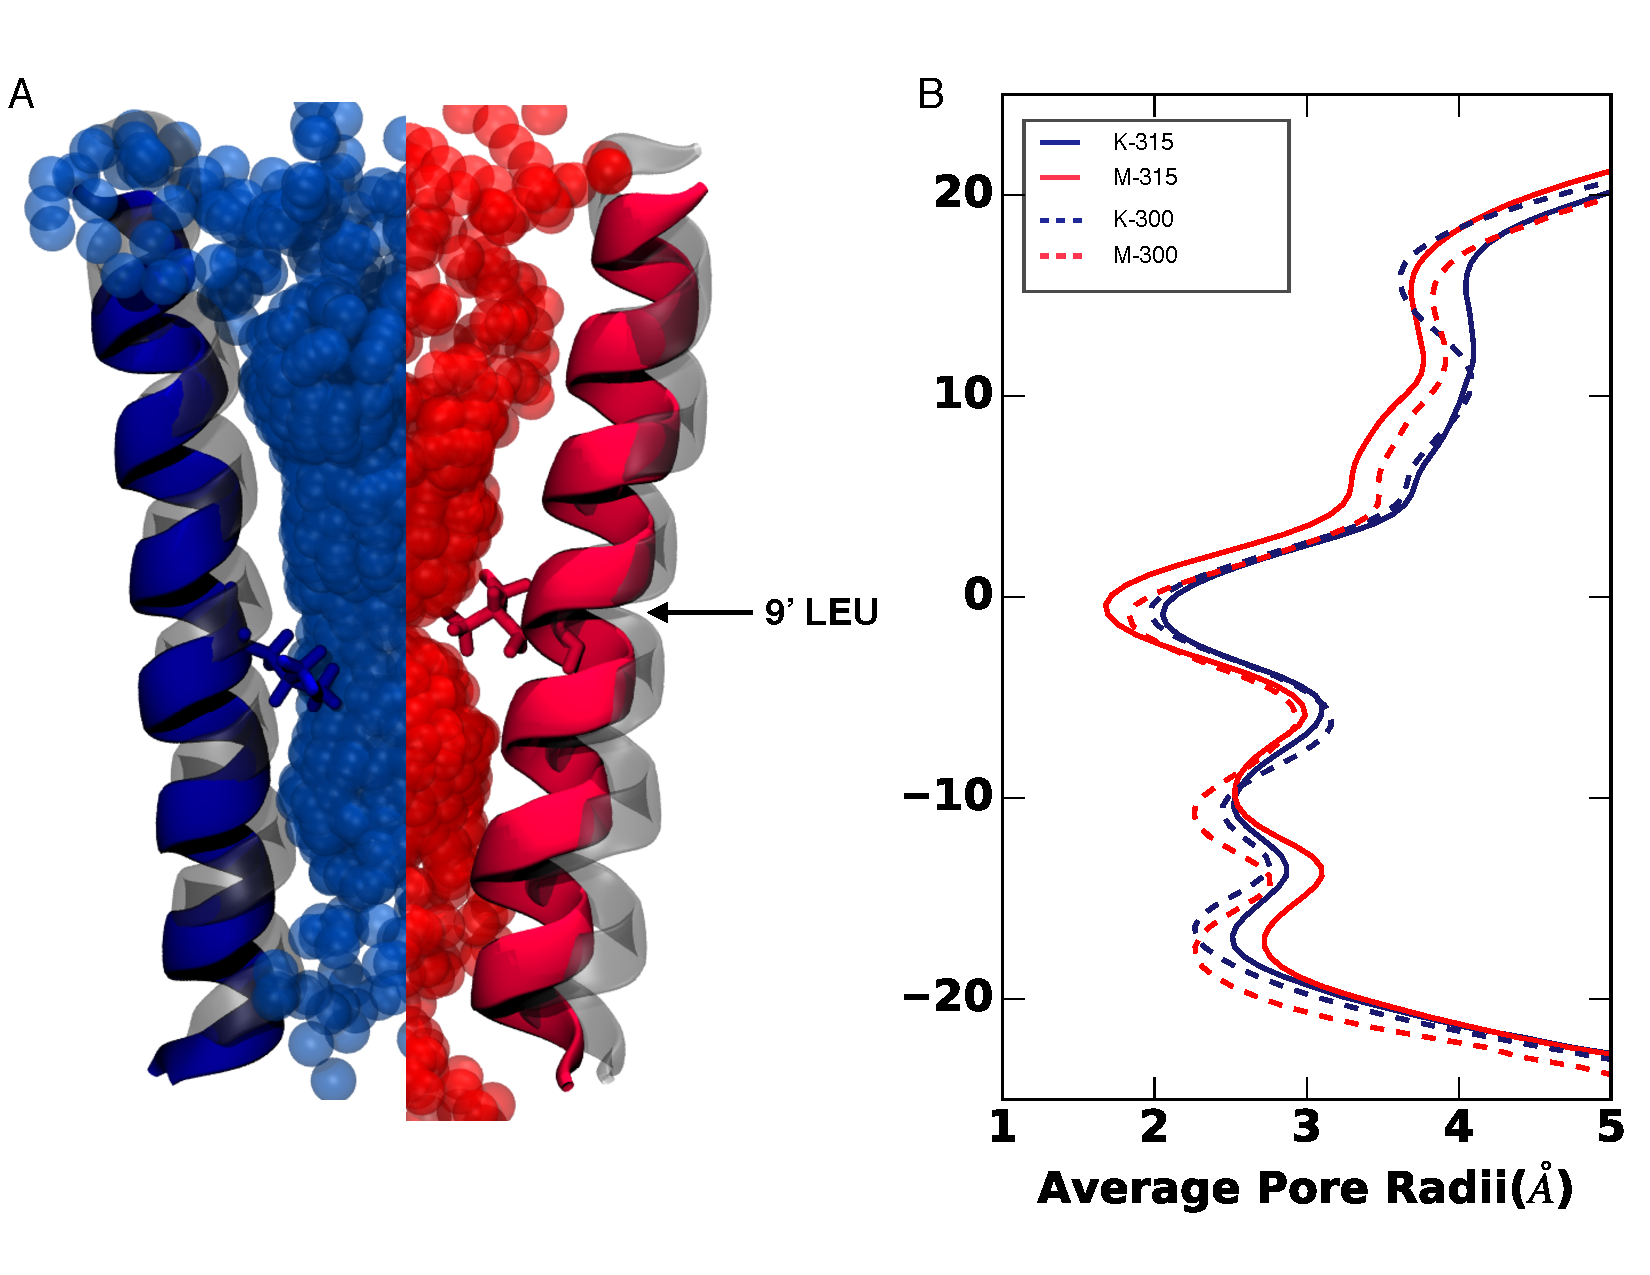
\includegraphics[width = .5\textwidth]{figures_2/pore_radd_fill.pdf}
%\end{center}
%\caption{(A) Comparison of pore radius profiles computed from simulations at 315 K, for \WT(blue) and \MT(red) conformations. (B) Pore radius along the pore axis, averaged over all frames and replicas, and at multiple temperatures. 
%}
%\label{fig:pore-profile}
%\end{figure}
%The mutation alone might also be expected to reduce stability of the open state of the channel, because the reduced charge \fivering becomes easier to shrink, regardless of temperature or shape. However, at the lower temperature, there is no effect of the mutation on the pore radius distribution (Figure \ref{fig:Pillar_3_fig} A).  As discussed under ``Predicted multibody interactions'',  it is also easier to shrink a distorted charged pentamer than a symmetric one, assuming the same total charge and average radius. Our results indicate that the distortion associated with the higher temperature, and allowed by the mutation, is necessary to shift the distribution of pore radii downward. This is consistent with the typical absence of seizures in individuals with this mutation, but without a fever, or with a fever but without the mutation.   

The \triadns-\fivering salt-bridge formation becomes uncorrelated from the pore radius in the \MT systems, as shown in Figure \ref{fig:Pillar_3_fig} F.  
%The cationic residue in the \triad is on the $\gamma$ subunit ($\gamma 285K$), and during relaxation of the \MT system, the charged end of $\gamma285K$ shifts toward the (now uncharged) sidechain of $\gamma$289 in the \fiveringnos.  The overall effect is to shift the \triadns, including the acidic residues, away from their salt-bridging partners in the rest of the \fiveringnos. %Forming the salt-bridges requires that the entire \fivering collapse around the \triadns. but this is not prohibitive in the \MT \fiveringnos. %because a separation of $r_{1}$ in the \MT system is equivalent to a separation of $5 r_{1}/3$ in the \WT system (i.e. $U_{+5}(5 r_{1}/3) = U_{+4}(r_{1})$). 
%Consequently, in the \MT system, salt-bridging between the \triad and \fivering has little effect on pore radius. 

% fluctuations in the shape of the \fivering were much larger for the \MT systems at 315K than any of the other systems, and the associated distribution is very (Figure \ref{fig:Pillar_3_fig} D).  
 %Qualitatively, a more open pore was correlated with a more symmetric \fiveringnos, which we characterized via the ratio of average diagonal/adjacent distances in the \triadns,  
 %Qualitative comparison of pore-radius vs \fivering symmetry within the same trajectories (Figure \ref{fig:Pillar_3_fig} Panel C vs A, or Panel D vs B) indicates a closed pore is correlated with an asymmetric \fivering (value for diagonal/adjacent $<<1/\phi$ indicates a concave \fiveringnos. while diagonal/adjacent $>> 1/\phi$ indicates an elongated \fiveringnos. This is consistent with the relatively low cost to shrink a concave or convex charged pentagon compared to a regular pentagon, as discussed in the Theory. The observed shift in pore radius with formation of two  \fivering-\triad salt bridges (Figure \ref{fig:Pillar_3_fig} Panel E) is removed in the mutant.  This suggests that the coupling between temperature and the \MT mutation is likely due to destabilization of the open state by distortion of the \fiveringnos.  
 
 %These trends mimic the overall reduction in the \fiveringnos. %GB: statistics?  
 % The open state of the channel is more stable when the pentamer is symmetric with distance/diagonal ratio  being close to 1.62. As the temperature increases (Figure \ref{fig:Pillar_3_fig} D), the open state of \WT system is more stabilized as the ratio approaches 1.62, while the opposite trend is visible in the \MT. The symmetry of the +5 charges is stabilized following the flip of $\alpha$ K279 towards the pore and the consistent formation of salt-bridge involving $\beta$ K274 and $\beta$ E270. While in the \MT the  $\beta$ K274 flip creates a more irregular pentagon thus not supporting the formation of proper salt-bridges (Figure \ref{fig:Pillar_3_fig} E,F),. 
 
\subsection*{$\gamma$ K289M increases barriers to conduction via channel conformation rather than direct interactions with ions}  
 
Determining whether a single ion channel conformation corresponds to an ``open'' or ``closed'' state is frequently not possible in unbiased MD simulations, except for conformations at an extremum. A Cl- atom has a radius of approximately 1.8\AA, the hydrophobic residues lining the minimum pore radius but makes it unlikely a Cl- atom will pass through a constriction of exactly 1.8\AA\ ; when both salt bridges between the \fivering and \triad are formed, the \WT receptor has a minimum pore radius of at least 2.5\AA.
%At 300K,  the minimum pore radius is greater than 1.8\AA\ for 69\% (\WT) and 43\% (\MT) of the frames, %SRUTHI - please check these numbers again
%while at 315K, the minimum pore radius is greater than 1.8\AA\ for 69\% (\WT) and 26\% (\MT) of the frames. 

The effects of the mutation on purely electrostatic barriers for chloride ion translocation was quantified via the Poisson-Boltzmann equation as described in SI Methods.  The mutation from a positively charged to neutral residue led to insignificant changes in the electrostatic potential along the most favorable path given identical starting conformations (as shown in Supplementary Figure S12), suggesting that the mutation alone could not affect conductance without inducing conformational shift. Although the electrostatic potential is weakened near the mutation, the ion can adjust its pathway through the channel to fall closer to the other four residues in the \fiveringnos. 
%However, these differences were very small compared to those observed (Figure S2(B)) after equilibration of the \WT and \MT receptors to the distinct conformations discussed in the previous section.  
Calculation of the electrostatic potential using the equilibrated structures of \WT and \MT receptors showed a 5-10 kcal/mol (Figure S12C) higher electrostatic barrier in \MT , predominantly occurring in the transmembrane domain enclosing the residues containing the minimum pore constriction region. 

The PMF for chloride ion translocation at 315K, measured using ABF, is shown in Figure \ref{fig:abf}. The largest barrier for the \WT of 8~kcal/mol is proximal to the leucine residues at M2 9$^{\prime}$, forming the tightest constriction; this barrier is increased by 5 kcal/mol for the mutant receptors. 
%The secondary electrostatic barrier closer to the mutation in Figure S5 is not clearly reflected in the PMF.  
The difference in PMF near residue $\gamma_{2} 289$ is much less than 1 kcal/mol. %A slight, broad well (relative to a reference position outside the receptor) is apparent around residue 289 in the PMF for the \WT receptor, while at the same location in the \MT receptor the PMF is slightly elevated relative to the reference location.  However, these differences are slight compared to the effects of the mutation on the primary barrier, indicating that 
While mutation of a positively charged to neutral residue does have a small effect on affinity of the chloride ion for the region of the receptor near the mutation, 
the dominant effect of the mutation on conduction is via conformational instability of the open state.  %The \fivering for the \WT receptor is in an \extended conformation for most of these calculations. 
%\cleardoublepage

\section*{CONCLUSION}
The primary new insights of this work are:  
\begin{enumerate}
\item Repulsive cross-pore electrostatic interactions at the TMD-ECD interface (the ``\fiveringnos'') stabilize the open state of the GABA(A) receptor; the \fivering becomes more resistant to shrinking as the average separation between adjacent charges decreases or as the relative strength of diagonal interactions is reduced. 
\item In \GABAA receptors with 2 $\alpha$ subunits, 2 $\beta$ subunits, and 1 $\gamma$ subunit, a three-body charge-dipole arrangement (the ``\triadns'') among three M2 helices (two adjacent and one diagonal) %at $20^{\prime}$ between homologous pore-facing  cationic and anionic residues on adjacent M2 helices and the homologous anionic residue on a diagonal M2 helix 
drives fluctuations in minimum pore radius, by alternating between a repulsive and an attractive configuration.  All three charges are conserved within $\alpha, \beta$ and $\gamma$ species of the GABA(A) receptor (although $\gamma_3$ has an arginine instead of a lysine, Figure \sfigAlignment).
\item Switching from an asymmetric to symmetric configuration of the interfacial residues in (1) can lock the charge-dipole interaction in (2) in a repulsive configuration, via a pair of salt-bridges between the \triad and \fiveringnos.   
\item Neutralizing one of the residues from (1), as in the epilepsy-associated $\gamma_{2}$K289M mutations, makes the cost to shrink the \fivering more sensitive to dispersion of the remaining charges; at higher temperatures this results in a significant population of closed states.  This is consistent with the flickering observed in receptors with this mutation in {\it vitro}, as well as the critical role of fever in inducing seizures for this phenotype. 
\end{enumerate}

The debate over the mechanism through which binding of a ligand at one site regulates the effects of binding of a ligand at another site (``allostery'') is over fifty years old,\cite{Changeux2011,Changeux2016} %https://www.ncbi.nlm.nih.gov/pmc/articles/PMC3169905/ 
 and much of that debate was focused on placing mechanisms within two extreme cases :  "conformational selection" (functional conformations are visited in the absence of ligand but stabilized by ligand, the Monod-Wyman-Changeux or MWC model)  or "induced fit"   (functional conformations require all ligands to be bound, also known as the Koshland-Nemethy-Filmer model).  
 
 The mechanism for pore opening observed here fits most consistently with an MWC model, but % We find a charge-dipole oscillator in the pore-lining helices of the GABA(A) heteropentamer that predicts pore occlusion surprisingly well, and which fluctuates through open and closed conformations over nanoseconds until a pronounced conformational change in one of the subunits stabilizes it in a ``latched'' open state.  Nonetheless, the mechanism by which the conformation is selected (the Flip step), involving a pronounced conformational change.%TEMP: is made more likely at higher temperature.
the presence of both the \fivering (1) and the \triad (2) suggests a sequence of conformational events, with each event in the sequence falling at a different location along the continuum between pure conformational selection and pure induced fit.  Although effects of the substitutions of  \fivering residues have been studied numerous times, we are unaware of mutagenesis studies involving either of the residues of the \triad ($\gamma K/R285$ and $\beta E270$).  The present simulation results suggest a role for these residues in determining receptor kinetics, including desensitization. 

%Cover Letter : The traditional formulation of the debate reflects an underlying question about how allosteric phenomenon violate a common expectation that significant interactions among subunits will be short-range and primarily at the subunit-subunit interface.  The results we present here indicate that this expectation on its own may be misguided, because the symmetry imposed by quaternary structure can significantly amplify the contribution of long-range electrostatic interactions to the energetic cost of a conformational change.  

%The reliance of current MD simulation software on approximate long-range electrostatics using methods such as Particle Mesh Ewald may contribute to the challenges in maintaining a stable open state even in the appropriate pH or in the presence of ligand; we comment further on this issue in SI Methods. 

Our results indicate that a topological view of pLGICs may be counterproductive for conceptualizing gating mechanisms, because interactions entirely within a helix/subunit (or between two adjacent helices/subunits) are only indirectly related to conformation of the pore.  %Considering pLGICs as a tower of stacked pentameric slices perpendicular to the pore axis, with certain residues moving from one slice into another depending on a signal propagating down the pore axis, may prove more useful.  
%They also emphasize the importance of considering the effective distance between two residues of a protein when considering the likelihood of significant interactions;  two distant charged residues are effectively much closer to each other than two hydrophobic residues at the same distance.  
While we present these results in heteropentamers, and the presence of the \triad requires multiple subunit species, the role of symmetry in stabilizing conformations with open or occluded pores has been demonstrated previously in both heteropentamers such as nAChR\cite{Mitra2005} and homopentamers such as GLIC. \cite{Mowrey2013} Our results indicate a critical role for diagonal interactions in determining the effects of asymmetry; asymmetry that decreases or increases diagonal distances opens or closes the pore respectively.  %beyond providing balancing interactions on either side of a subunit, particularly in the case of repeated charged residues. %, but through its role in determining repulsions or attractions of the numerous charged rings formed by repeated charged residues.  

%Lastly, while these simulations alone cannot directly illuminate the ligand-gating mechanism, they inspire a clear hypothesis in which binding of each of two ligands causes rearrangement of the extracellular domain, reducing the energetic cost of one or two of the initial Flip steps, upon which the receptor continues the sequence in Figure \ref{fig:finalcartoon}.  This would be consistent with previous simulation results\cite{Lev2017} finding breaking of salt-bridges between the GLIC ECD and residues of the homologous GLIC \fivering along the pathway to an open state, as well as the numerous experimental results identifying the critical role of such salt-bridges in eukaryotic pLGICS.      

More generally, the Coulomb interaction between two charges placed on the diagonal of a regular pentagon will only be moderately reduced from the interaction they would have as adjacent charges. Diagonal interactions will always contribute $38\%$ of the overall interaction energy.  A role for long range interactions within the \nachr TMD-ECD interface has been recently demonstrated by Auerbach and colleagues\cite{Gupta2017}.  The residues forming an \fivering  need not be located in the M2-M3 loop; they could also be in the M1 linker as in nAChR, or even in the M4 C-terminus.  The concept of an \fivering that we propose here is topologically abstract, but depends on pentameric symmetry and a regular charge density at the interface between the two domains; it may therefore be generalizable to many or even all \plgics.    %This result holds regardless of the distance of the charges (or residues) from the pentagon (or pore) center, but does require pentameric symmetry.  %For any particular \plgic , we can conclude that {\emph {any} charged residues conserved across subunits} will contribute to stabilizing an open pore.  Such residues may be in the M1 linker in some heteromeric \plgics (a role for long range interactions within the \nachr TMD-ECD interface has been recently demonstrated by Auerbach and colleagues\cite{Gupta2017}) and in the M2-M3 loop in other heteromeric \plgics (such as \GABAA).    %Any charged residue in a homomeric pLGIC will have this property at a pH for which nearly all of the residues are charged. 
%This result suggests interesting possibilities for identification of residues critical to stabilizing open states in heteromeric pLGICs: charged residues that are conserved across all subunit species for a given channel, forming a charged pentagonal ring, regardless of their conservation in other \plgic sequences.    %For instance, a second mutation in $\gamma_{2}$ (R43Q\cite{Audenaert2006}) associated with benign febrile seizures is also in a charged ECD residue conserved within \GABAA subunits, and also adjacent to a proline (P44). The conformational flexibility introduced by the proline may amplify the effect of temperature, for both that mutation and the one studied here.

%while a second mutation also associated with febrile seizures (R138G) is in a residue charged only in $\gamma$ subunits, and associated with more rapid desensitization. \cite{Audenaert2006} %http://www.neurology.org/content/67/4/687 %Is R138 correct one? Think it might be R176, also next to proline! because they say their R is conserved and R138 really isn't.  

\section*{ACKNOWLEDGMENTS}
SM, RS, and GB were supported by research grants  NSF MCB1330728 and NIH P01GM55876-14A1. This project was supported with computational resources from the National Science Foundation XSEDE program through allocation NSF-MCB110149 as well as a local cluster funded by NSF-DBI1126052.  The authors are grateful to Dr. J\'{e}r\^{o}me H\'{e}nin for multiple useful discussions.  

%\cleardoublepage
\bibliographystyle{pnas-new.bst}
\bibliography{GABAa_K289M}
\end{document}